\section{Experiments}
\label{sec:experiments}

\subsection{Experimental Setup}
\label{subsec:experimental_setup}

We evaluate WindFormer on two SCADA-based wind farm datasets with distinct spatial layouts and wind regimes: Shanxi with 24 turbines and Penmanshiel with 14 turbines. Both datasets are sampled at 10-min intervals and preprocessed following the protocol in Section~\ref{sec:data_preprocessing_task}. Unless otherwise specified, the input window is 288 steps, corresponding to 48 h of history, and the forecasting horizons are 6, 12, and 18 steps.

\begin{figure}[htbp]
\centering

\includegraphics[width=0.8\textwidth]{figures/data.png}
\caption{Geographical visualization of the two wind farm datasets used in the experiments.}
\label{fig:dataset_geography}
\end{figure}

WindFormer is compared with MST-Net, PatchTST, TimeMixer++, GLPT, DLinear, TimesNet, and iTransformer. Mean absolute error (MAE) and root mean squared error (RMSE) are reported for wind speed (m/s) and wind direction (rad). The experiments are organized around four research questions: standard accuracy and efficiency (RQ1), component attribution (RQ2), robustness to perturbations and extreme volatility (RQ3), and transfer to unseen turbines (RQ4).

\subsection{RQ1: Does WindFormer Improve Forecasting Accuracy and Efficiency?}
\label{subsec:standard_forecasting}

The standard setting trains and tests on the full turbine set without artificial perturbation. We first compare the complete forecasting performance on the two wind farms, then examine direction-aware error profiles, computational cost, and matched-seed statistical consistency.

\begin{table}[htbp]
\caption{Detailed full-sample forecasting performance on the Penmanshiel dataset under the noise-free setting. Lower values indicate better performance.}
\label{tab:main_penmanshiel}
\centering
\scriptsize
\setlength{\tabcolsep}{5pt}
\renewcommand{\arraystretch}{1.04}
\begin{adjustbox}{max width=\textwidth}
\begin{tabular}{llcccccccc}
\toprule
Metric & Horizon & WindFormer & MST-Net & TimeMixer++ & iTransformer & PatchTST & TimesNet & GLPT & DLinear \\
\midrule
\multirow{3}{*}{Speed MAE} & 6 & \textbf{0.7142} & 0.7978 & 0.9229 & 0.9272 & 0.9189 & 0.9210 & 0.9318 & 0.9263 \\
& 12 & \textbf{0.8812} & 0.9879 & 1.1421 & 1.1491 & 1.1347 & 1.1406 & 1.1543 & 1.1473 \\
& 18 & \textbf{1.0103} & 1.1249 & 1.2994 & 1.3081 & 1.2891 & 1.2976 & 1.3138 & 1.3061 \\
\midrule
\multirow{3}{*}{Speed RMSE} & 6 & \textbf{1.1497} & 1.2162 & 1.3053 & 1.3118 & 1.2987 & 1.3033 & 1.3174 & 1.3108 \\
& 12 & \textbf{1.4211} & 1.5538 & 1.6162 & 1.6247 & 1.6054 & 1.6142 & 1.6325 & 1.6224 \\
& 18 & \textbf{1.6216} & 1.7599 & 1.8367 & 1.8477 & 1.8263 & 1.8348 & 1.8553 & 1.8447 \\
\midrule
\multirow{3}{*}{Direction MAE} & 6 & \textbf{0.1456} & 0.1637 & 0.1898 & 0.1911 & 0.1884 & 0.1894 & 0.1926 & 0.1939 \\
& 12 & \textbf{0.1881} & 0.2113 & 0.2439 & 0.2460 & 0.2403 & 0.2434 & 0.2483 & 0.2497 \\
& 18 & \textbf{0.2204} & 0.2471 & 0.2847 & 0.2872 & 0.2807 & 0.2840 & 0.2899 & 0.2913 \\
\midrule
\multirow{3}{*}{Direction RMSE} & 6 & \textbf{0.2914} & 0.3092 & 0.3314 & 0.3341 & 0.3294 & 0.3320 & 0.3354 & 0.3375 \\
& 12 & \textbf{0.3686} & 0.3905 & 0.4176 & 0.4213 & 0.4146 & 0.4184 & 0.4237 & 0.4260 \\
& 18 & \textbf{0.4244} & 0.4599 & 0.4796 & 0.4843 & 0.4761 & 0.4807 & 0.4870 & 0.4906 \\
\bottomrule
\end{tabular}
\end{adjustbox}
\end{table}

\begin{table}[htbp]
\caption{Detailed full-sample forecasting performance on the Shanxi dataset under the noise-free setting. Lower values indicate better performance.}
\label{tab:main_shanxi}
\centering
\scriptsize
\setlength{\tabcolsep}{5pt}
\renewcommand{\arraystretch}{1.04}
\begin{adjustbox}{max width=\textwidth}
\begin{tabular}{llcccccccc}
\toprule
Metric & Horizon & WindFormer & MST-Net & TimeMixer++ & iTransformer & PatchTST & TimesNet & GLPT & DLinear \\
\midrule
\multirow{3}{*}{Speed MAE} & 6 & \textbf{0.6367} & 0.7062 & 0.8192 & 0.8222 & 0.8165 & 0.8274 & 0.8270 & 0.8217 \\
& 12 & \textbf{0.8025} & 0.8939 & 1.0343 & 1.0395 & 1.0309 & 1.0452 & 1.0447 & 1.0379 \\
& 18 & \textbf{0.9309} & 1.0337 & 1.1970 & 1.2024 & 1.1953 & 1.2098 & 1.2094 & 1.2013 \\
\midrule
\multirow{3}{*}{Speed RMSE} & 6 & \textbf{0.9884} & 1.0377 & 1.1203 & 1.1248 & 1.1172 & 1.1320 & 1.1311 & 1.1242 \\
& 12 & \textbf{1.2374} & 1.3033 & 1.4035 & 1.4097 & 1.3986 & 1.4178 & 1.4167 & 1.4078 \\
& 18 & \textbf{1.4116} & 1.4862 & 1.6002 & 1.6073 & 1.5987 & 1.6172 & 1.6161 & 1.6059 \\
\midrule
\multirow{3}{*}{Direction MAE} & 6 & \textbf{0.2717} & 0.2984 & 0.3460 & 0.3478 & 0.3445 & 0.3507 & 0.3500 & 0.3516 \\
& 12 & \textbf{0.3441} & 0.3806 & 0.4403 & 0.4426 & 0.4384 & 0.4465 & 0.4459 & 0.4476 \\
& 18 & \textbf{0.4019} & 0.4437 & 0.5130 & 0.5160 & 0.5115 & 0.5206 & 0.5199 & 0.5223 \\
\midrule
\multirow{3}{*}{Direction RMSE} & 6 & \textbf{0.5530} & 0.5778 & 0.6225 & 0.6269 & 0.6210 & 0.6283 & 0.6273 & 0.6300 \\
& 12 & \textbf{0.6525} & 0.7041 & 0.7356 & 0.7409 & 0.7342 & 0.7454 & 0.7440 & 0.7471 \\
& 18 & \textbf{0.7275} & 0.7831 & 0.8196 & 0.8255 & 0.8184 & 0.8295 & 0.8285 & 0.8324 \\
\bottomrule
\end{tabular}
\end{adjustbox}
\end{table}

Tables~\ref{tab:main_penmanshiel} and \ref{tab:main_shanxi} show that WindFormer achieves the best wind-speed and wind-direction accuracy across all reported horizons on both datasets. The consistent ranking across terrain conditions and forecast lengths supports the central design choice of matching the representation to the physical structure of each variable.

\begin{figure}[htbp]
\centering
\setlength{\tabcolsep}{0pt}
\begin{tabular}{cc}
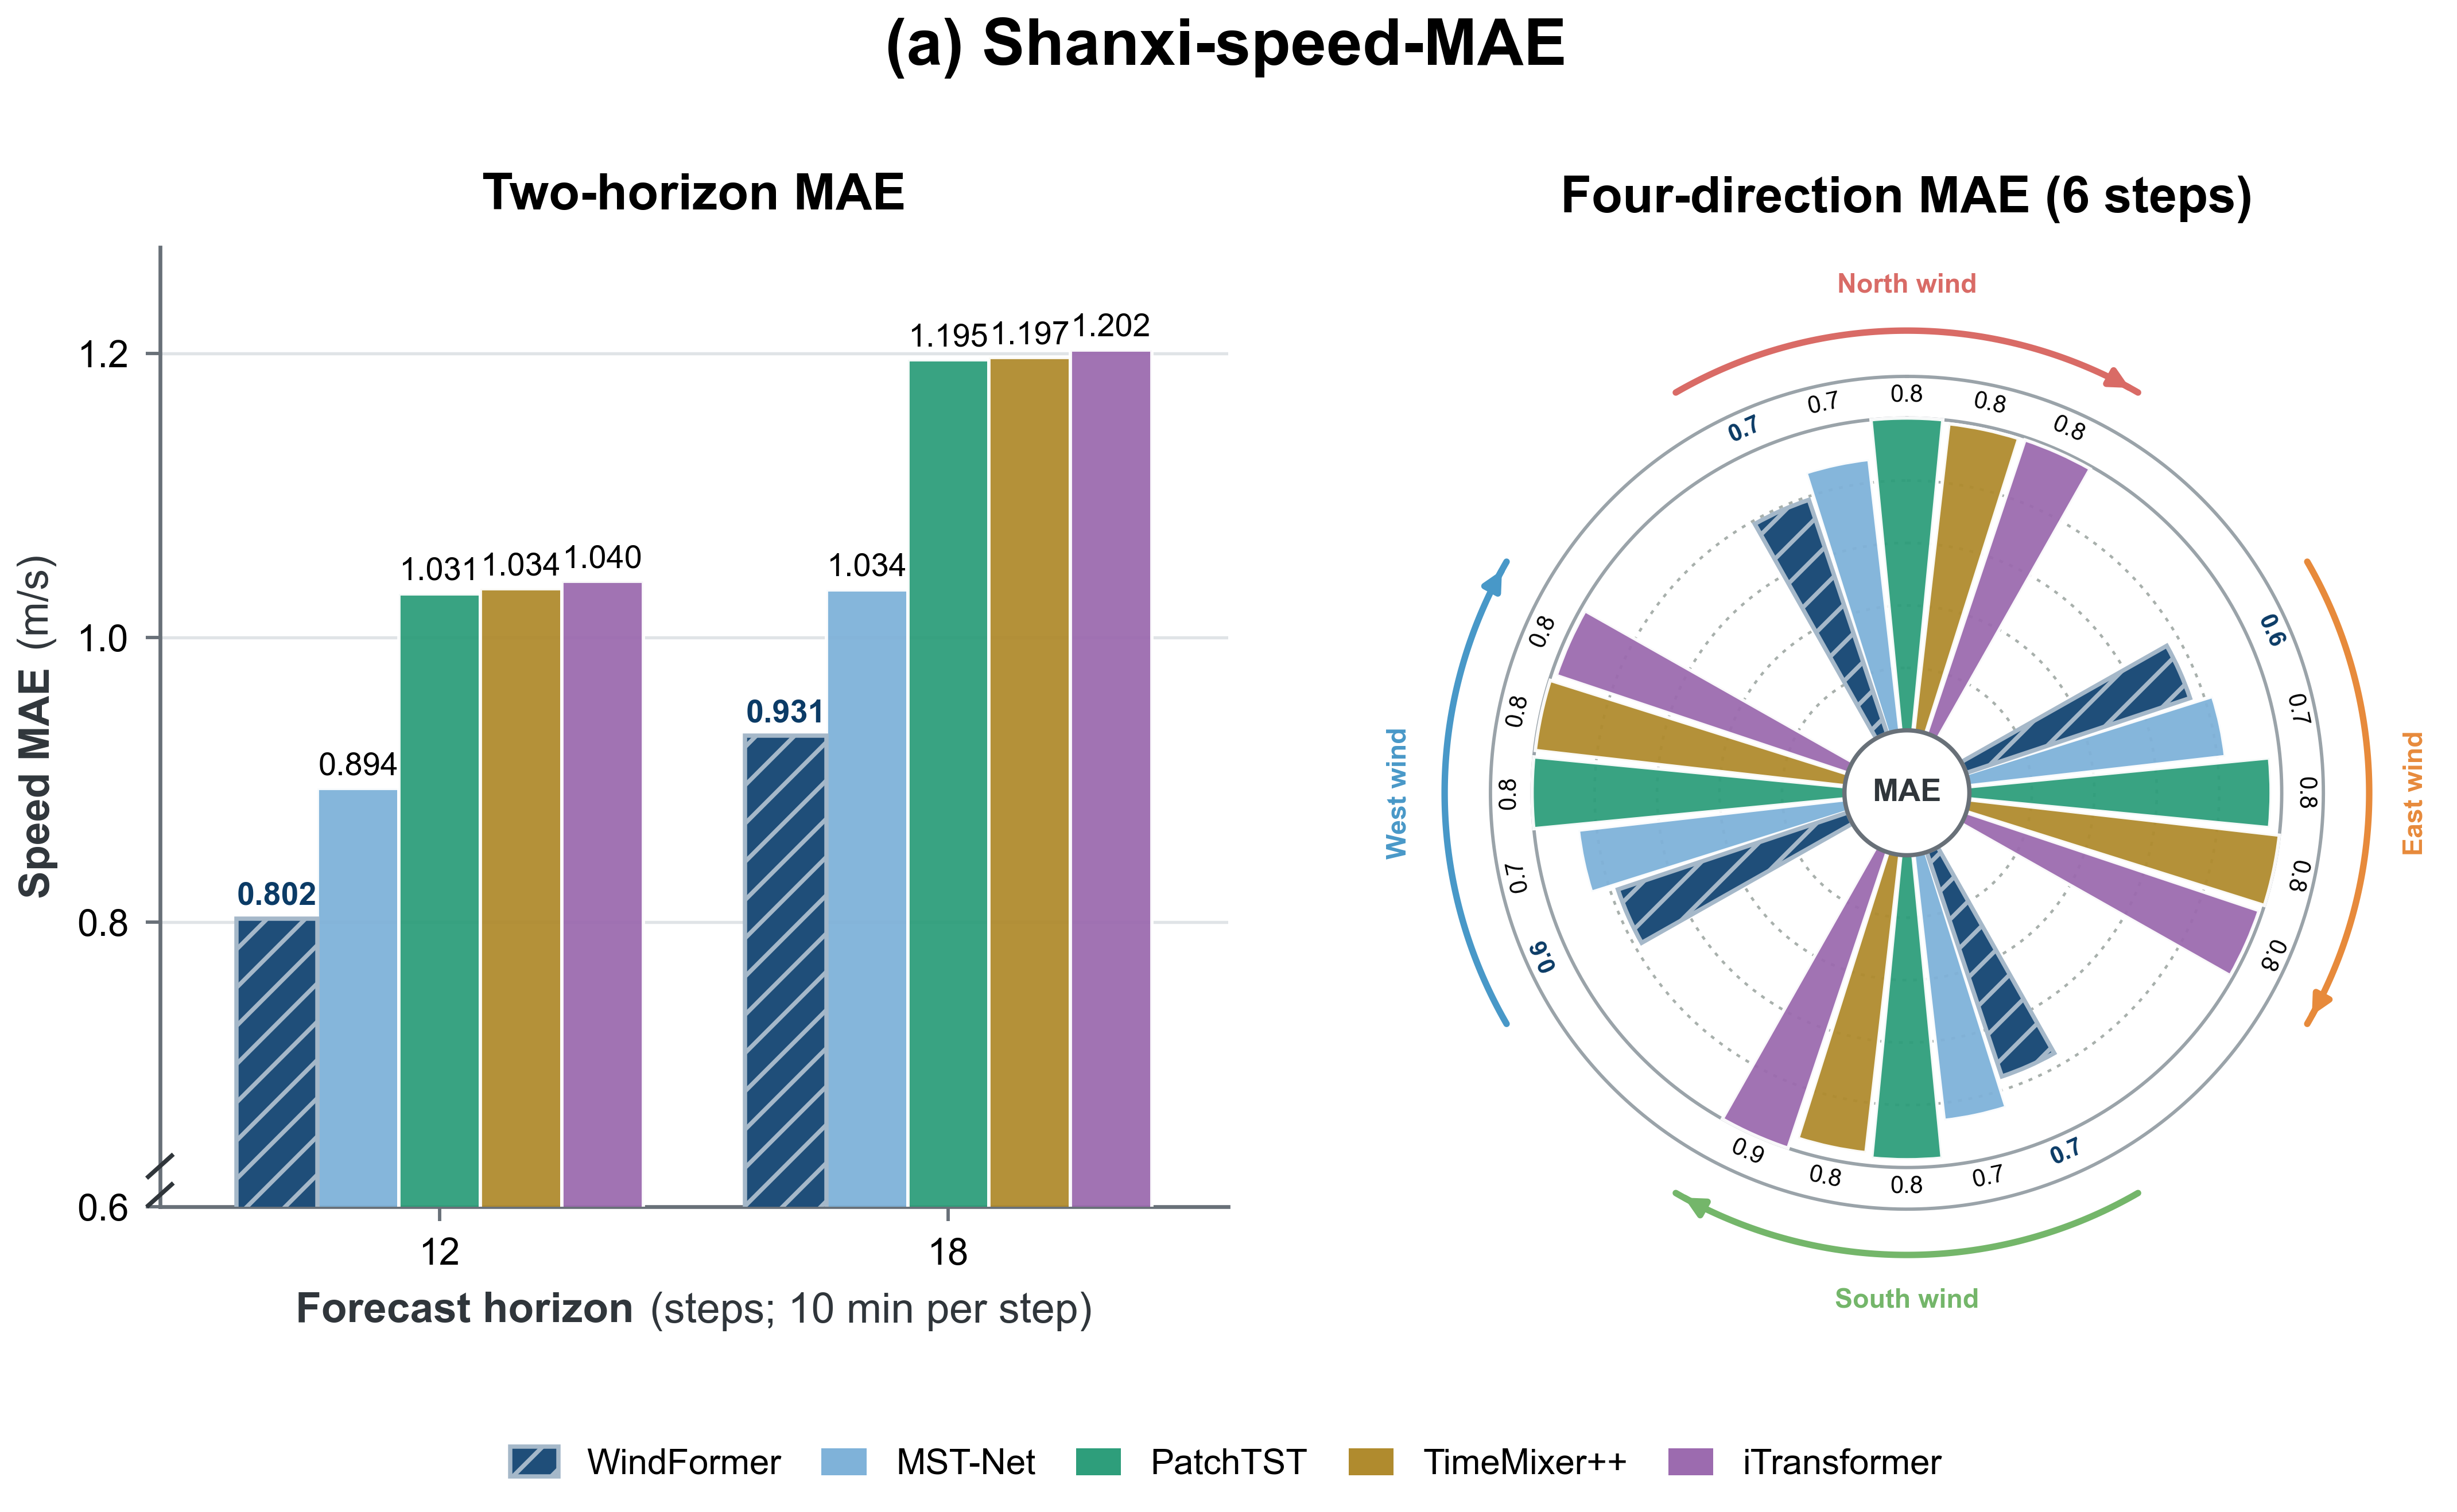
\includegraphics[width=0.49\textwidth]{figures/fig_shanxi_speed_mae.png} &
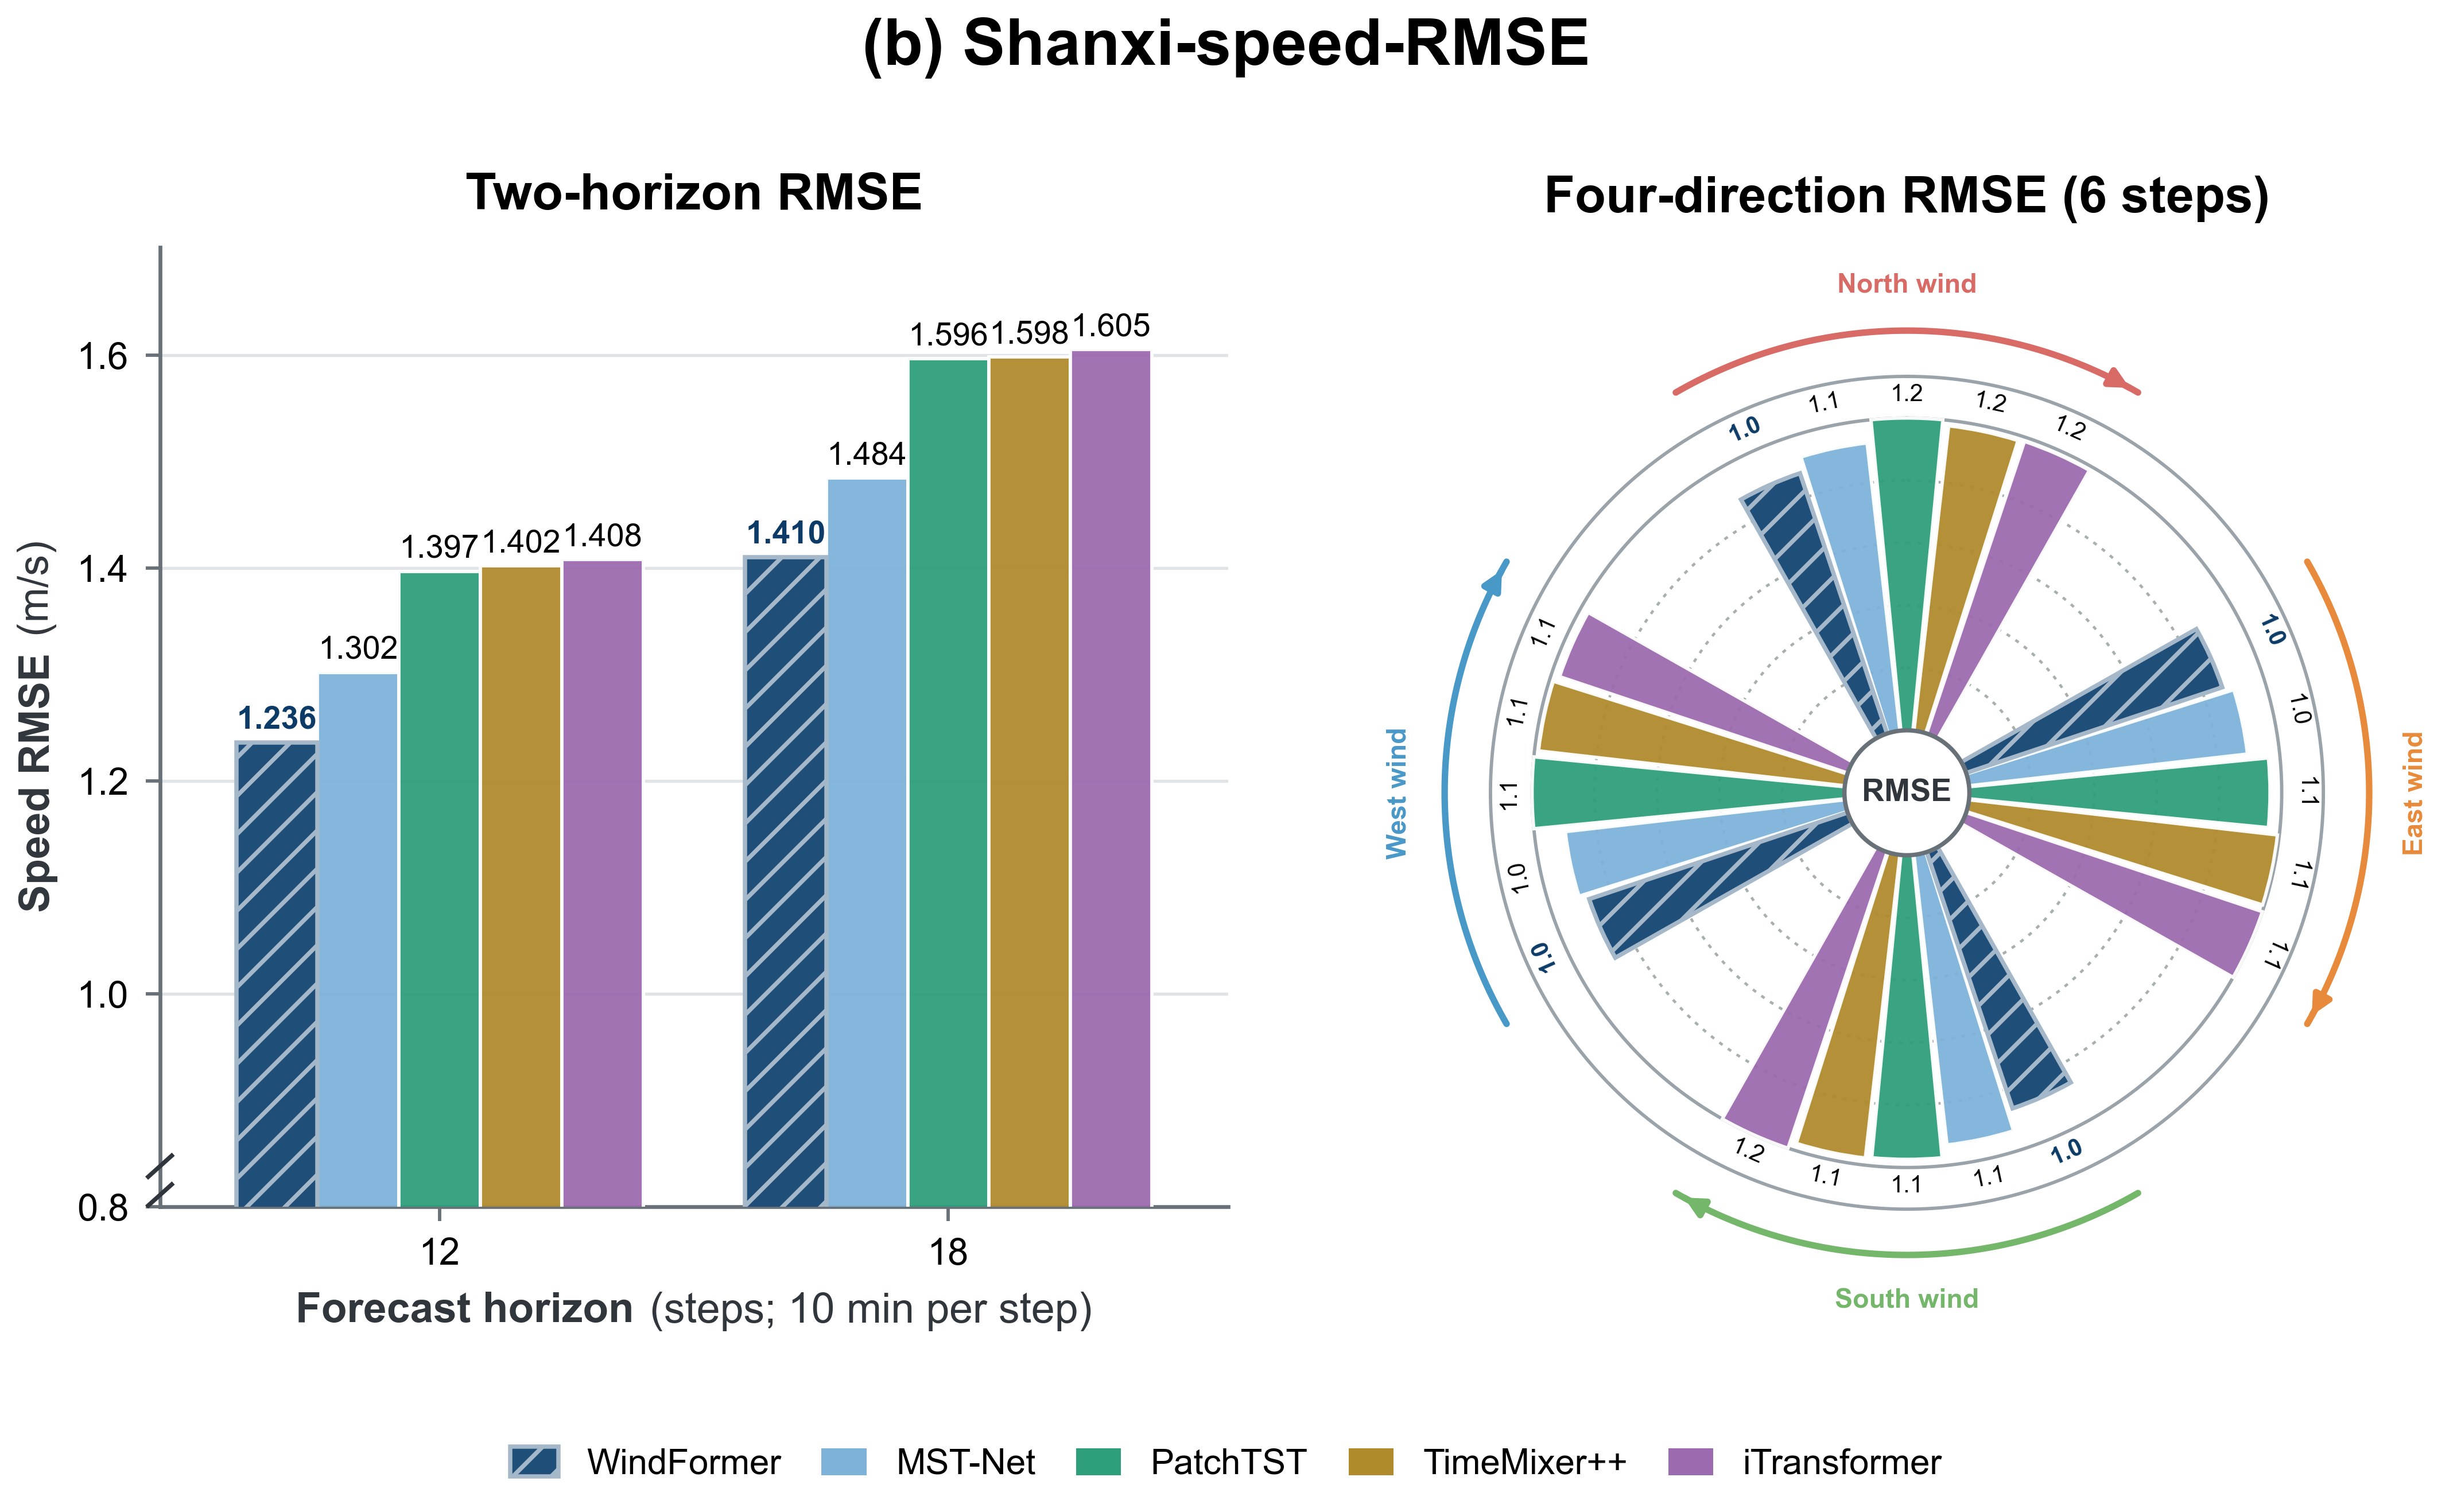
\includegraphics[width=0.49\textwidth]{figures/fig_shanxi_speed_rmse.png} \\[1pt]
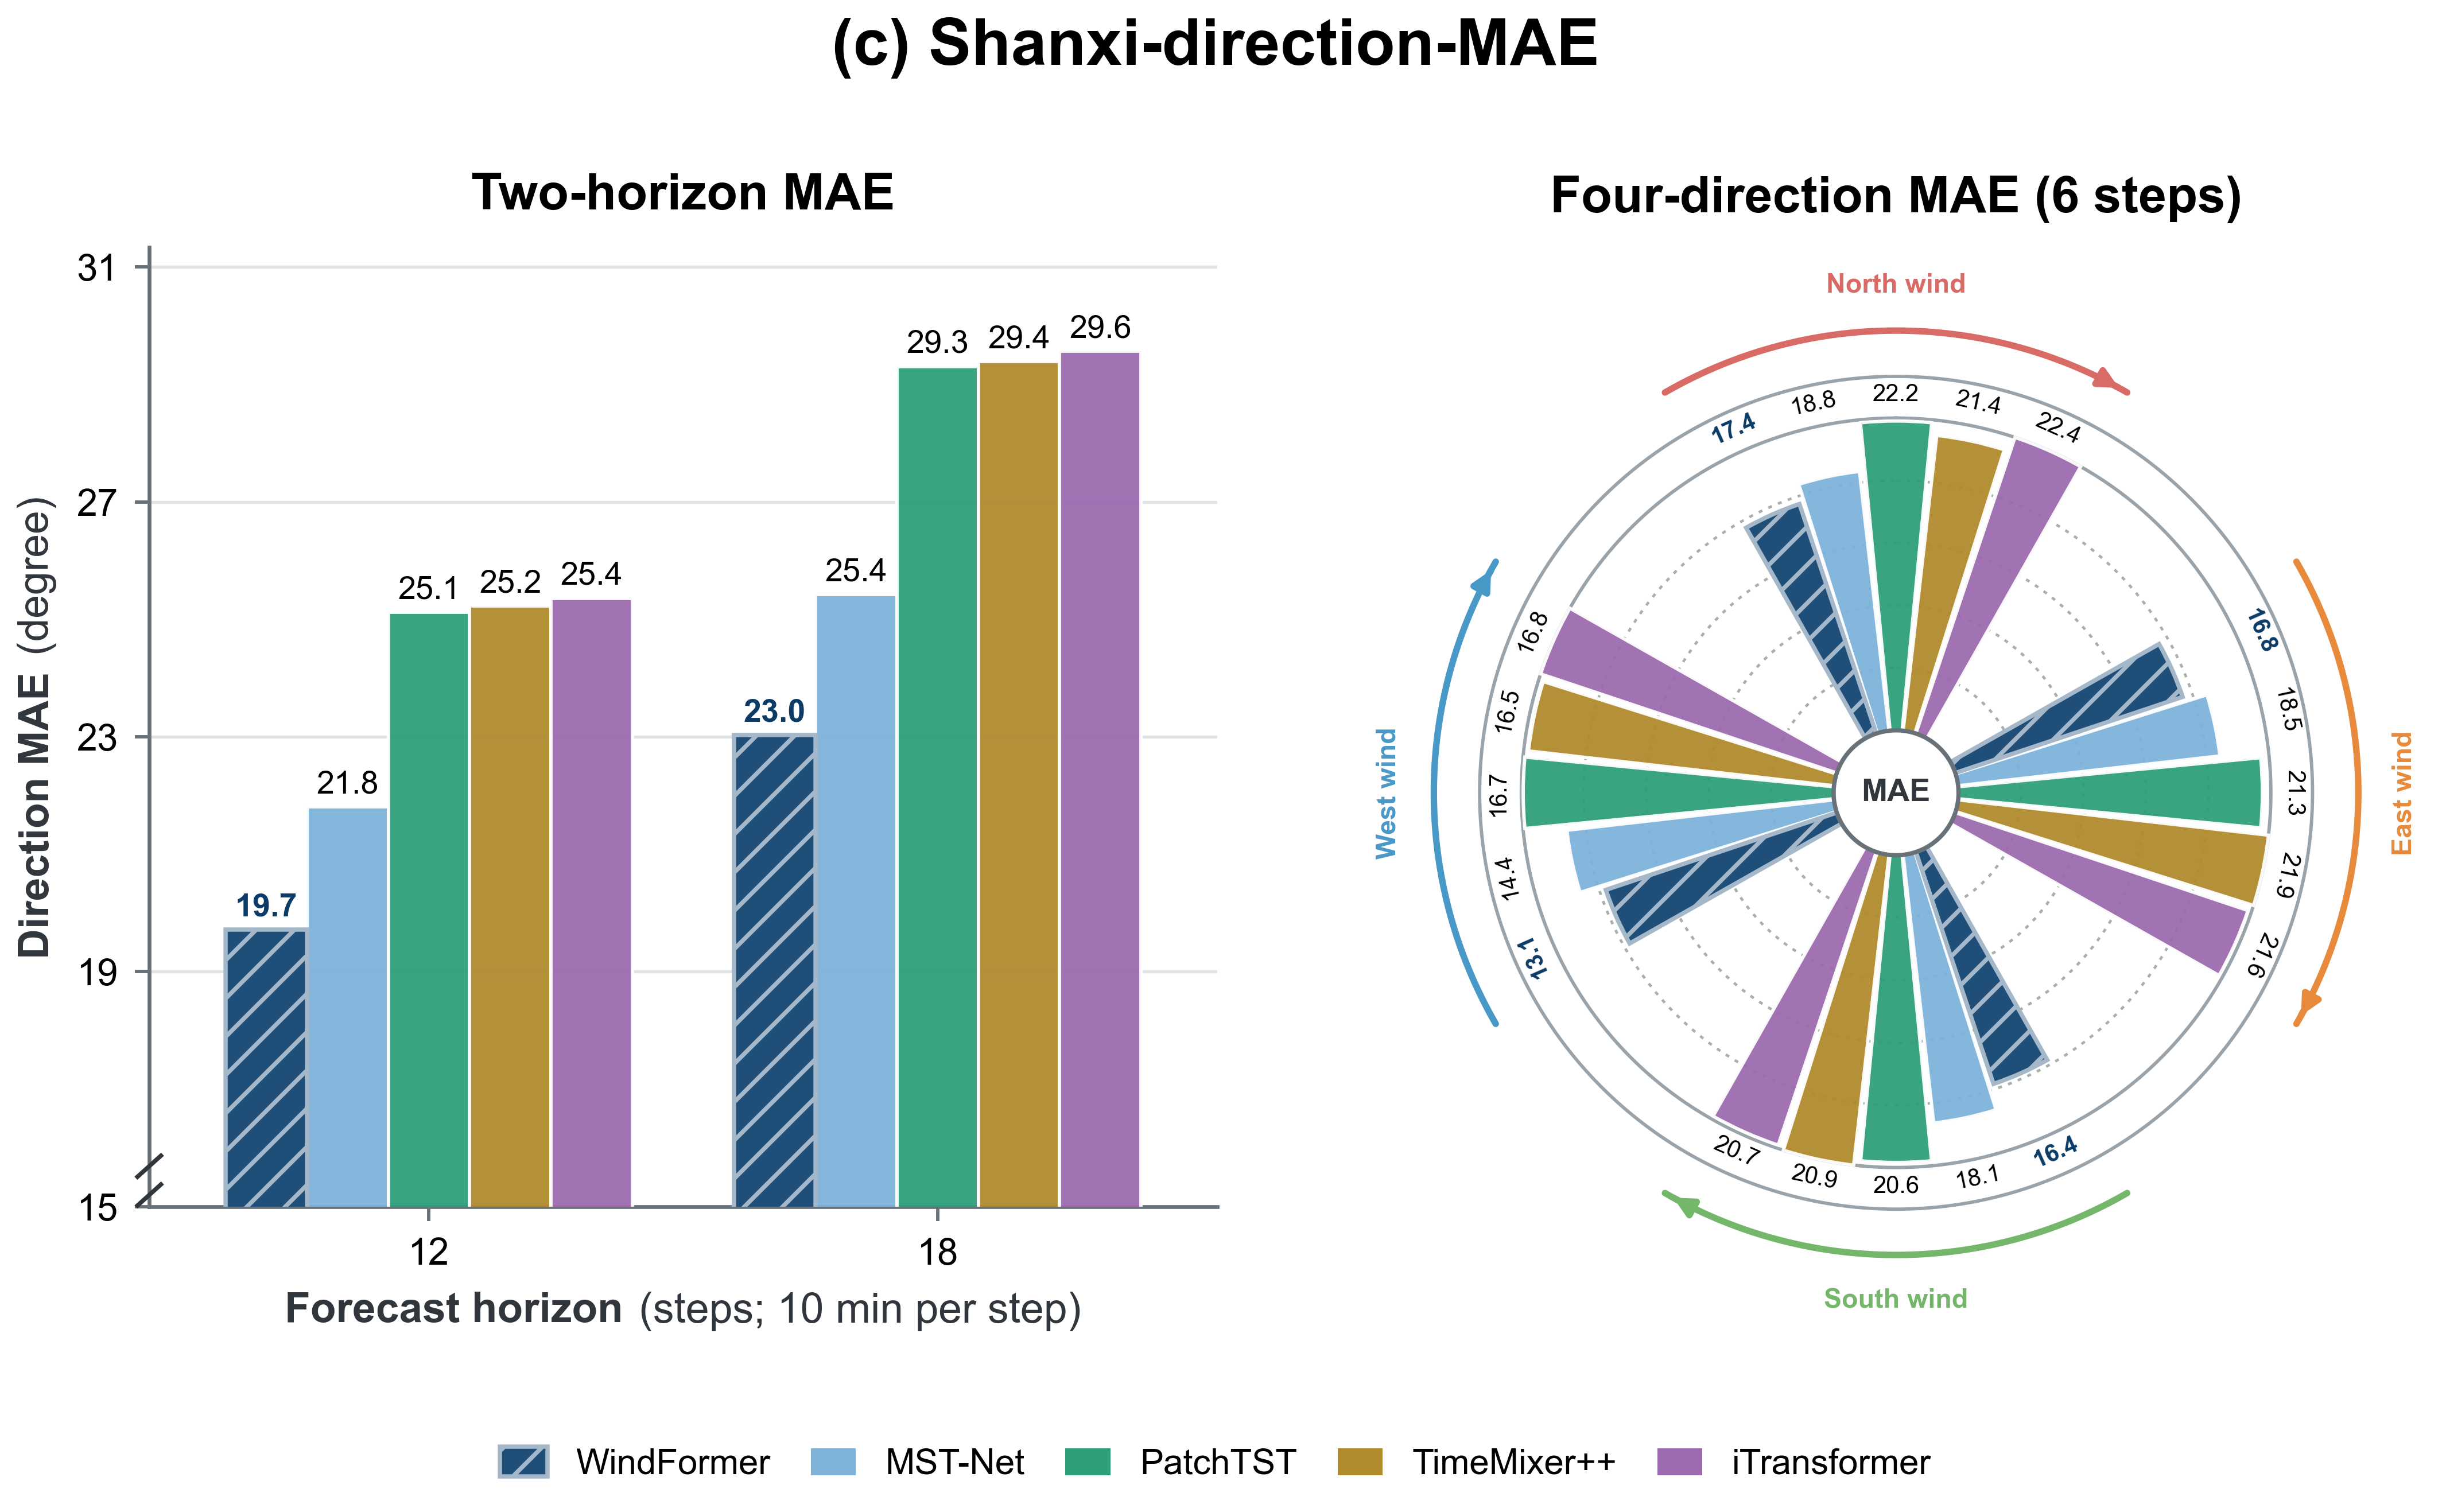
\includegraphics[width=0.49\textwidth]{figures/fig_shanxi_direction_mae.png} &
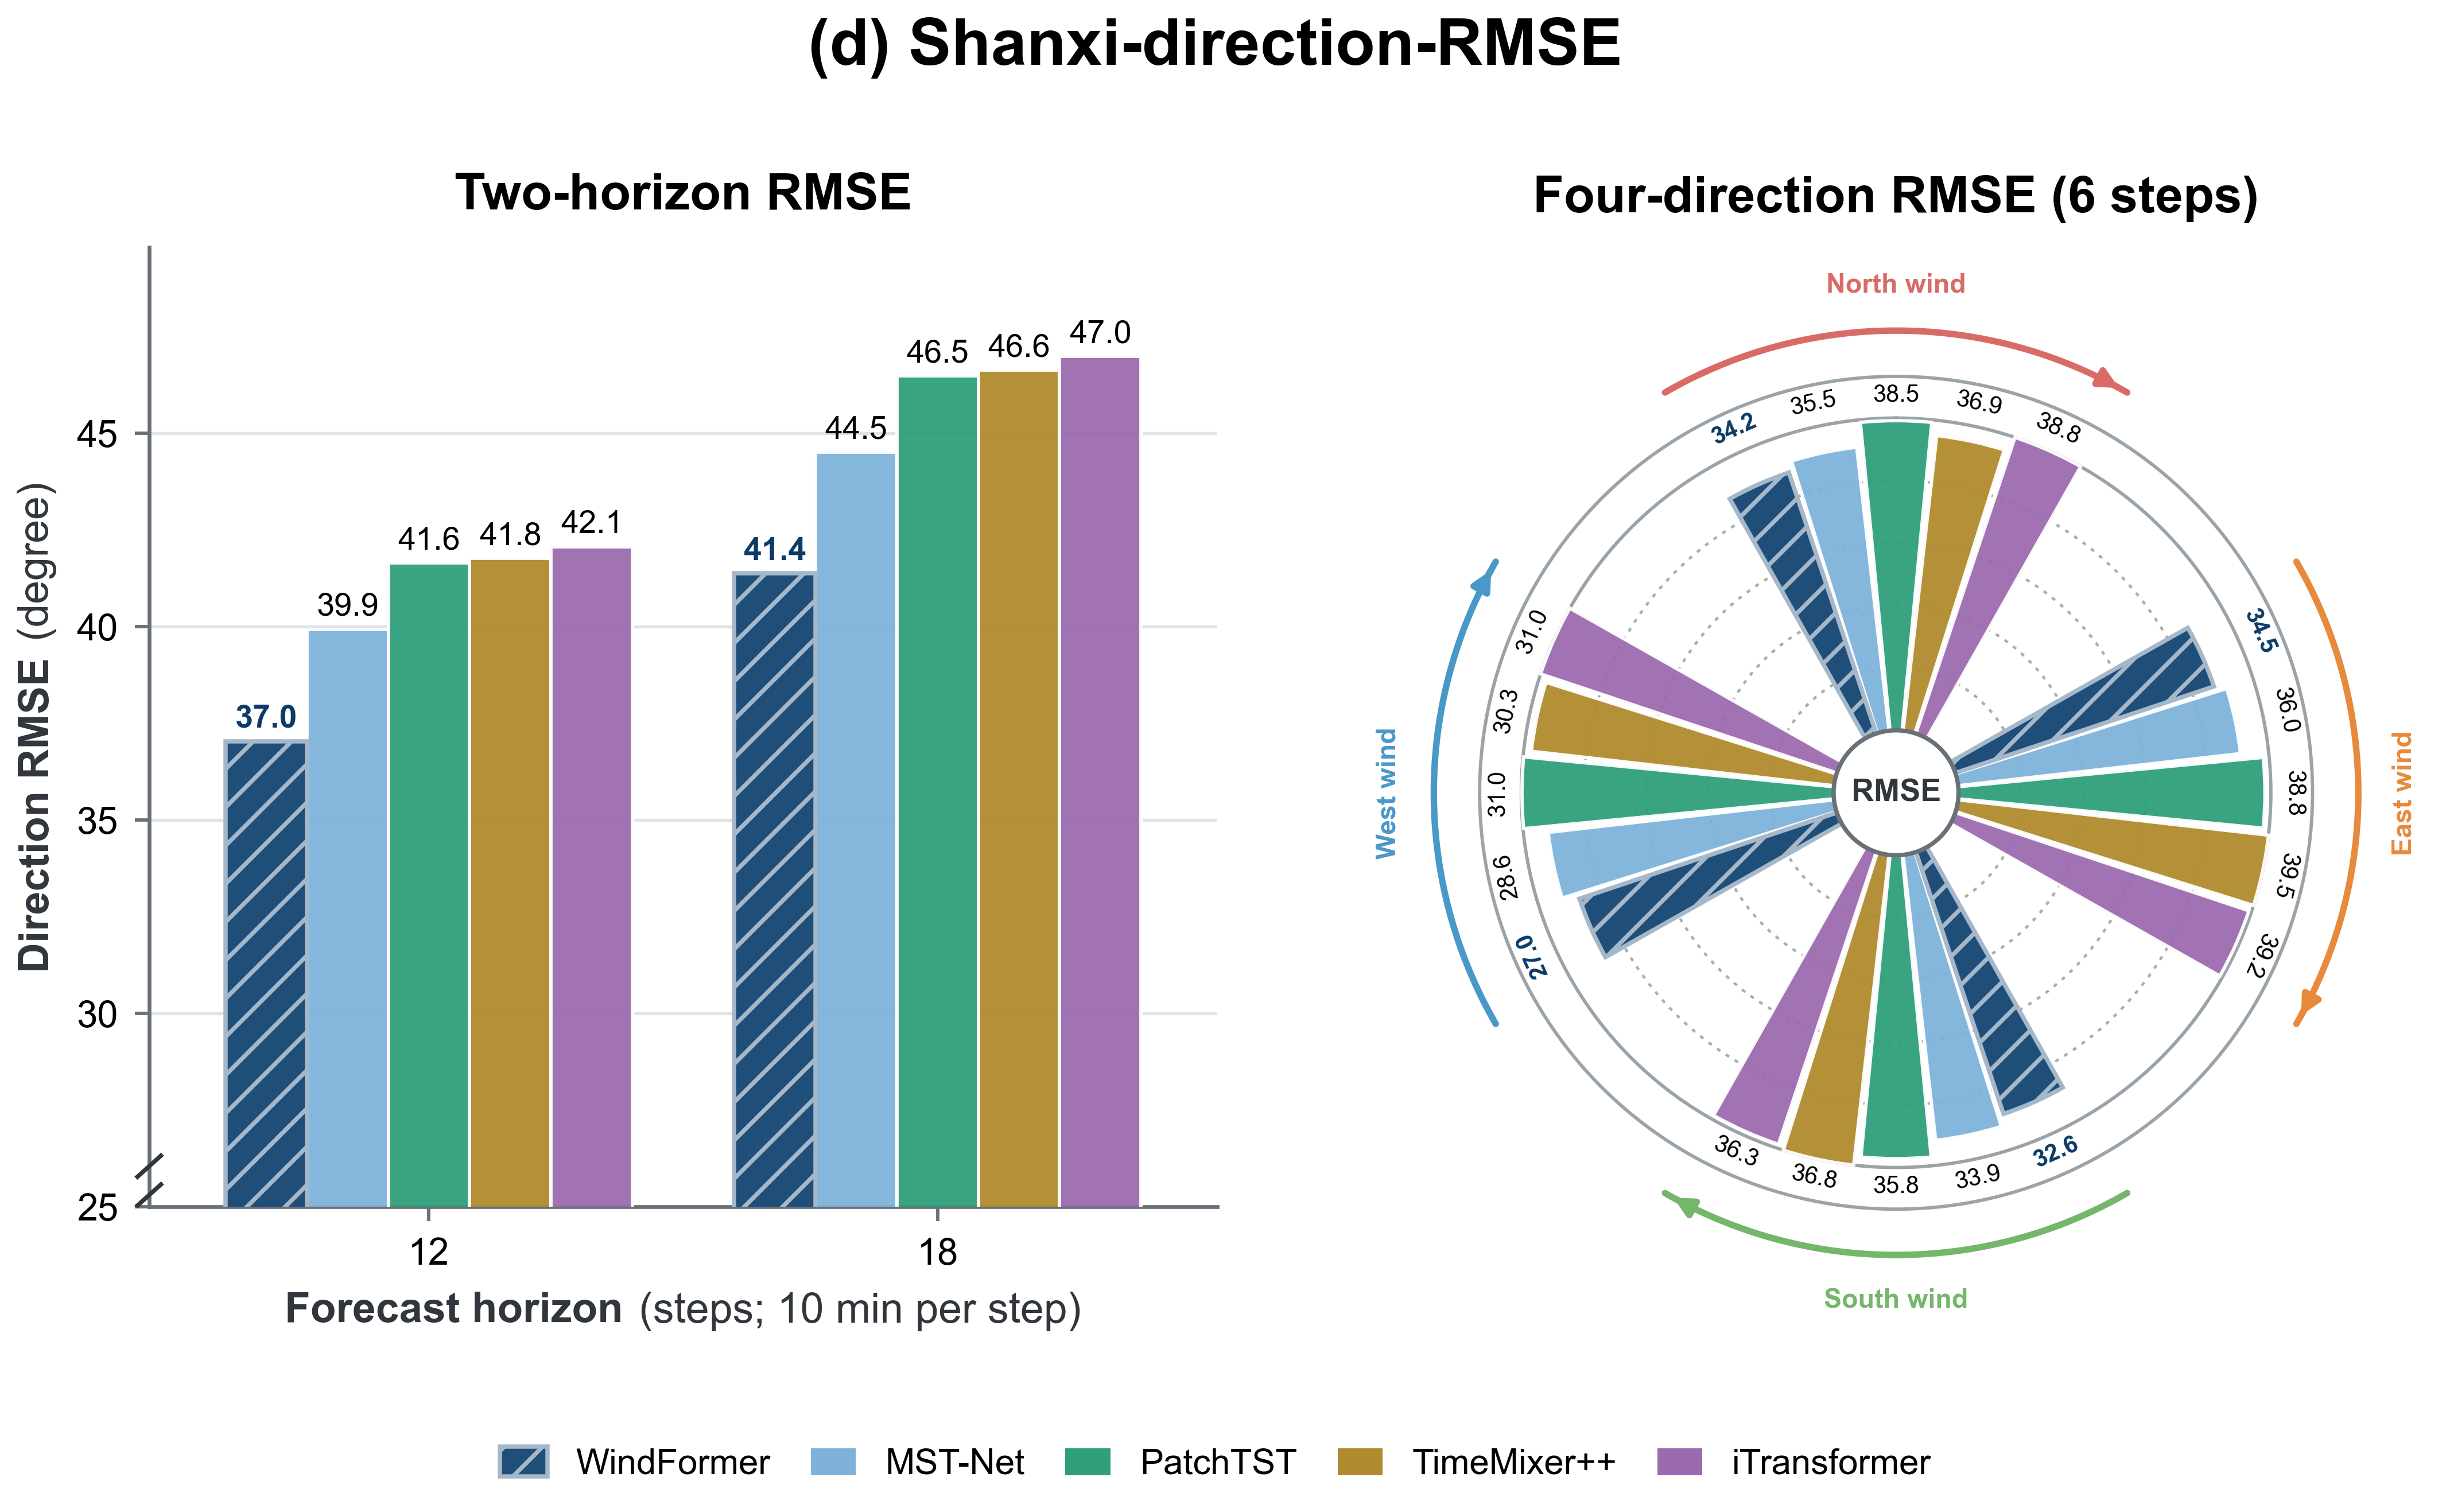
\includegraphics[width=0.49\textwidth]{figures/fig_shanxi_direction_rmse.png} \\[1pt]
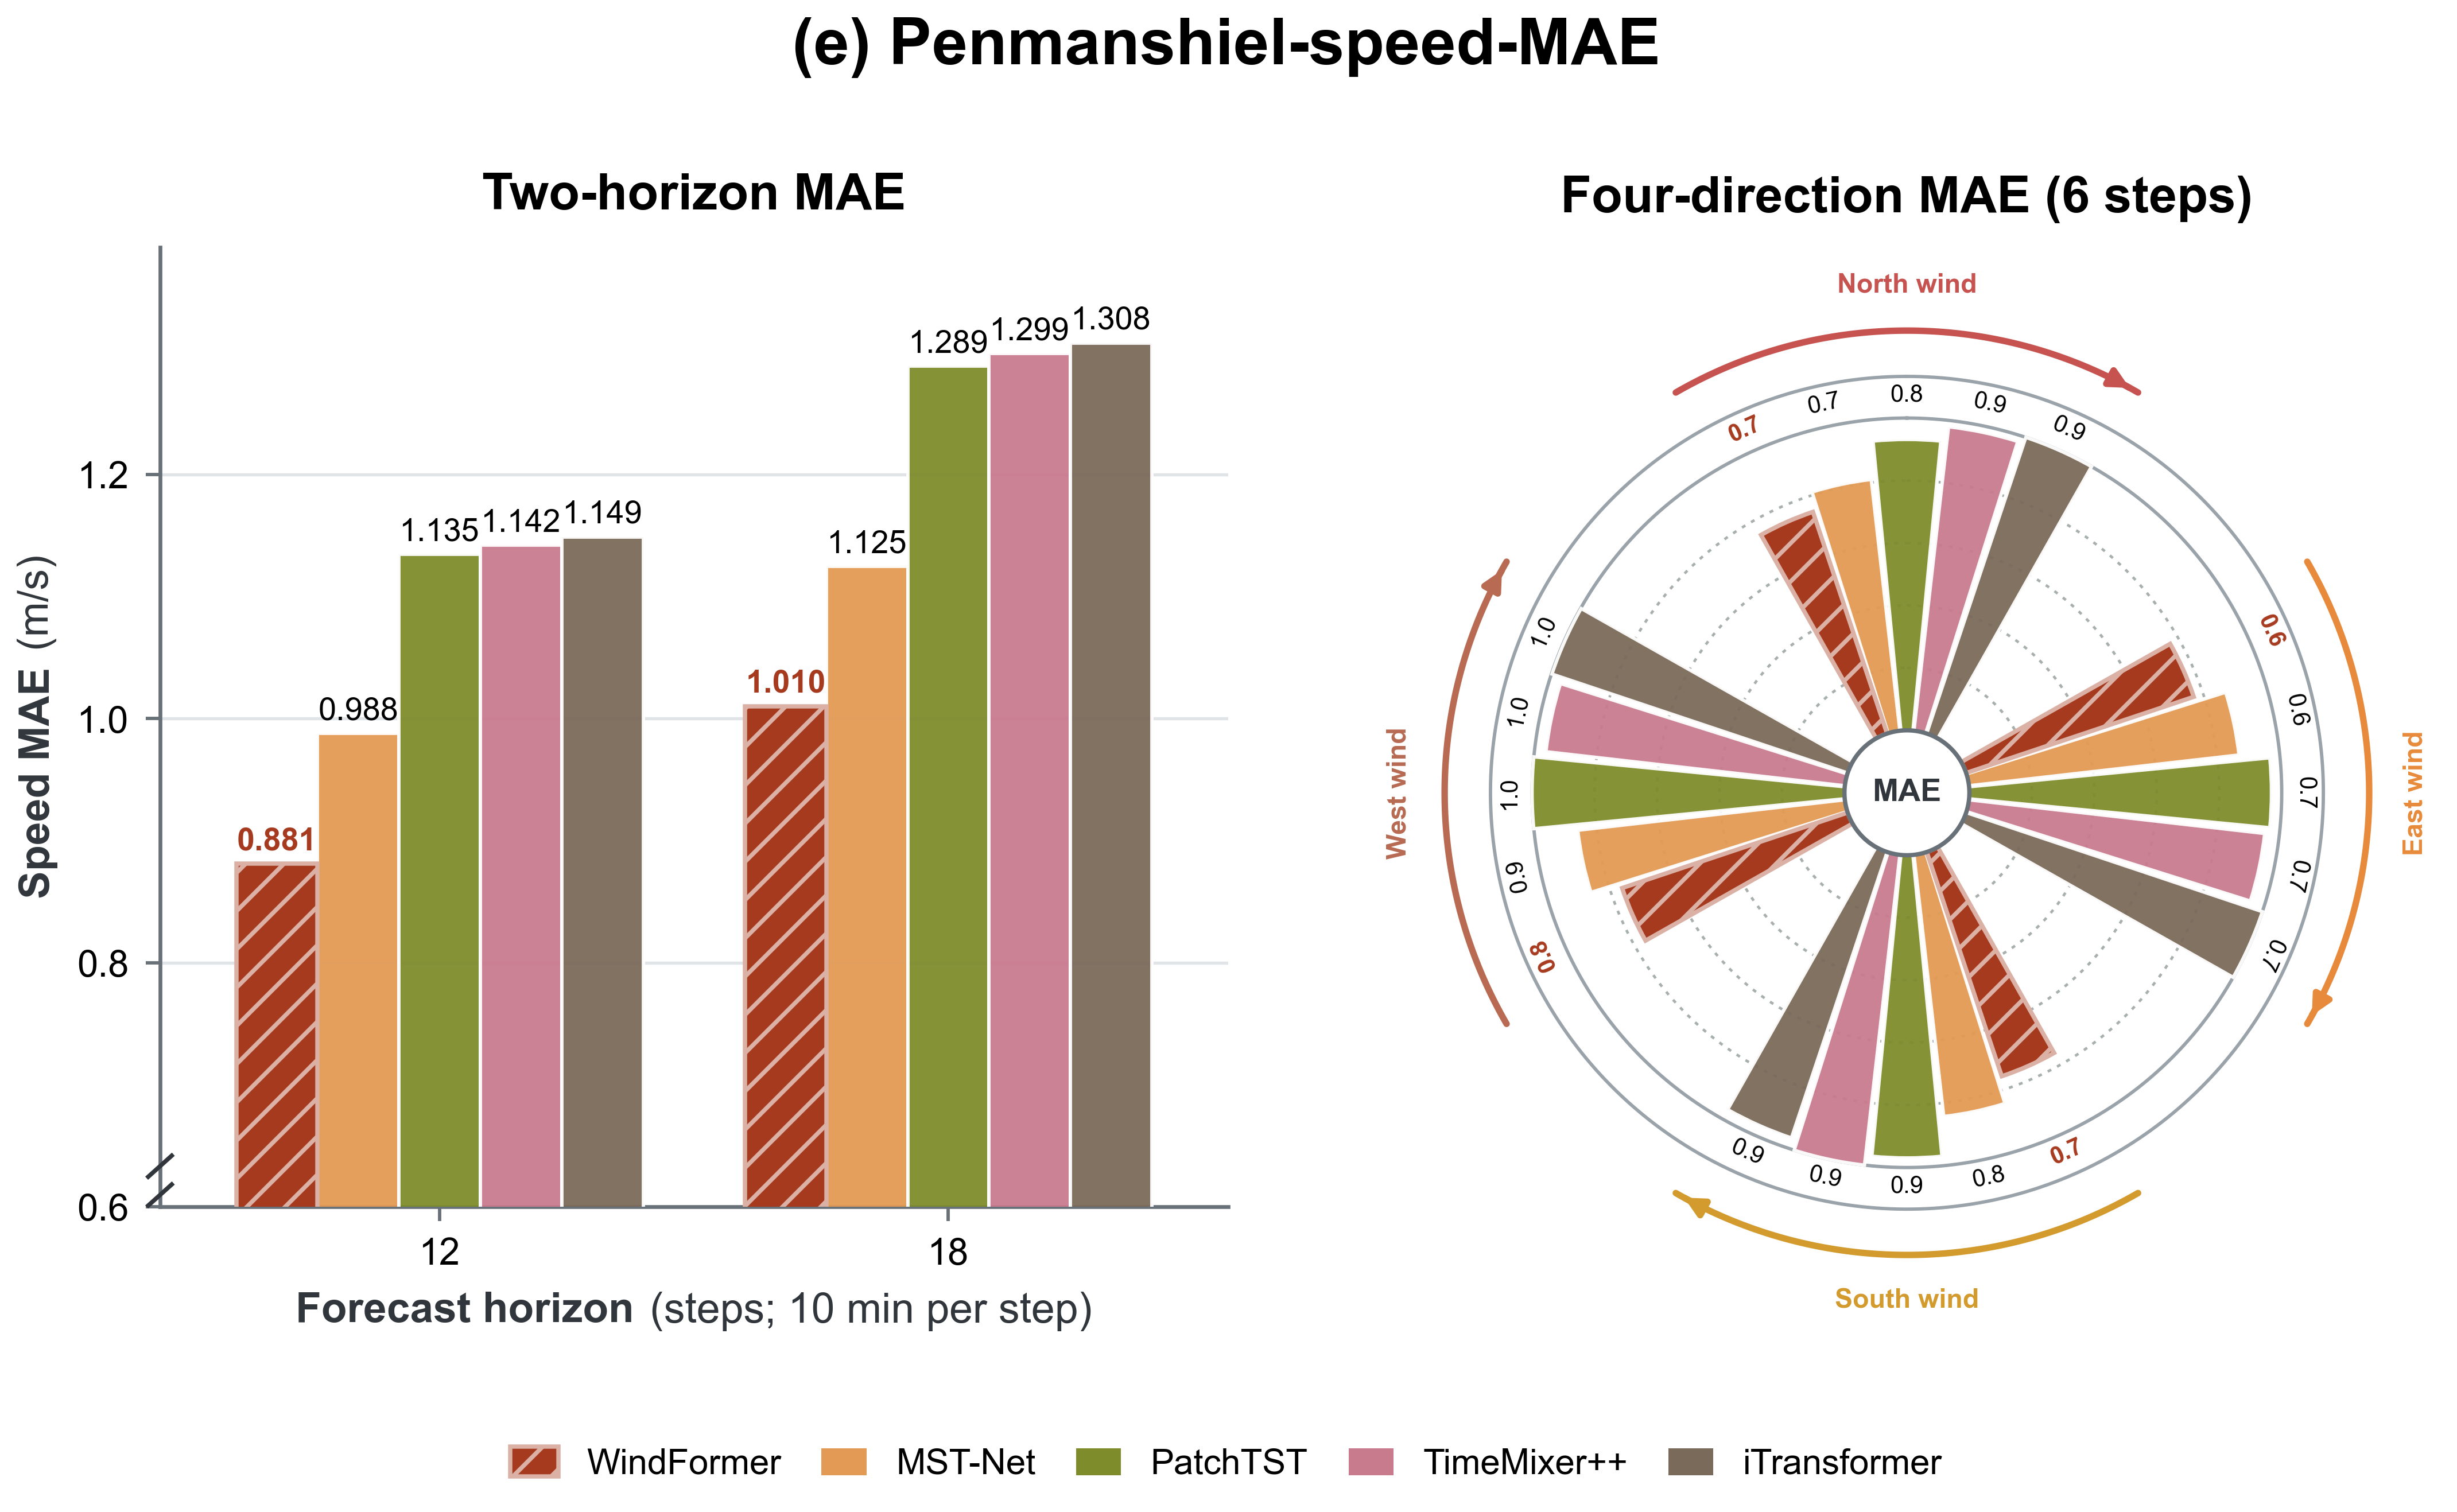
\includegraphics[width=0.49\textwidth]{figures/fig_penmanshiel_speed_mae.png} &
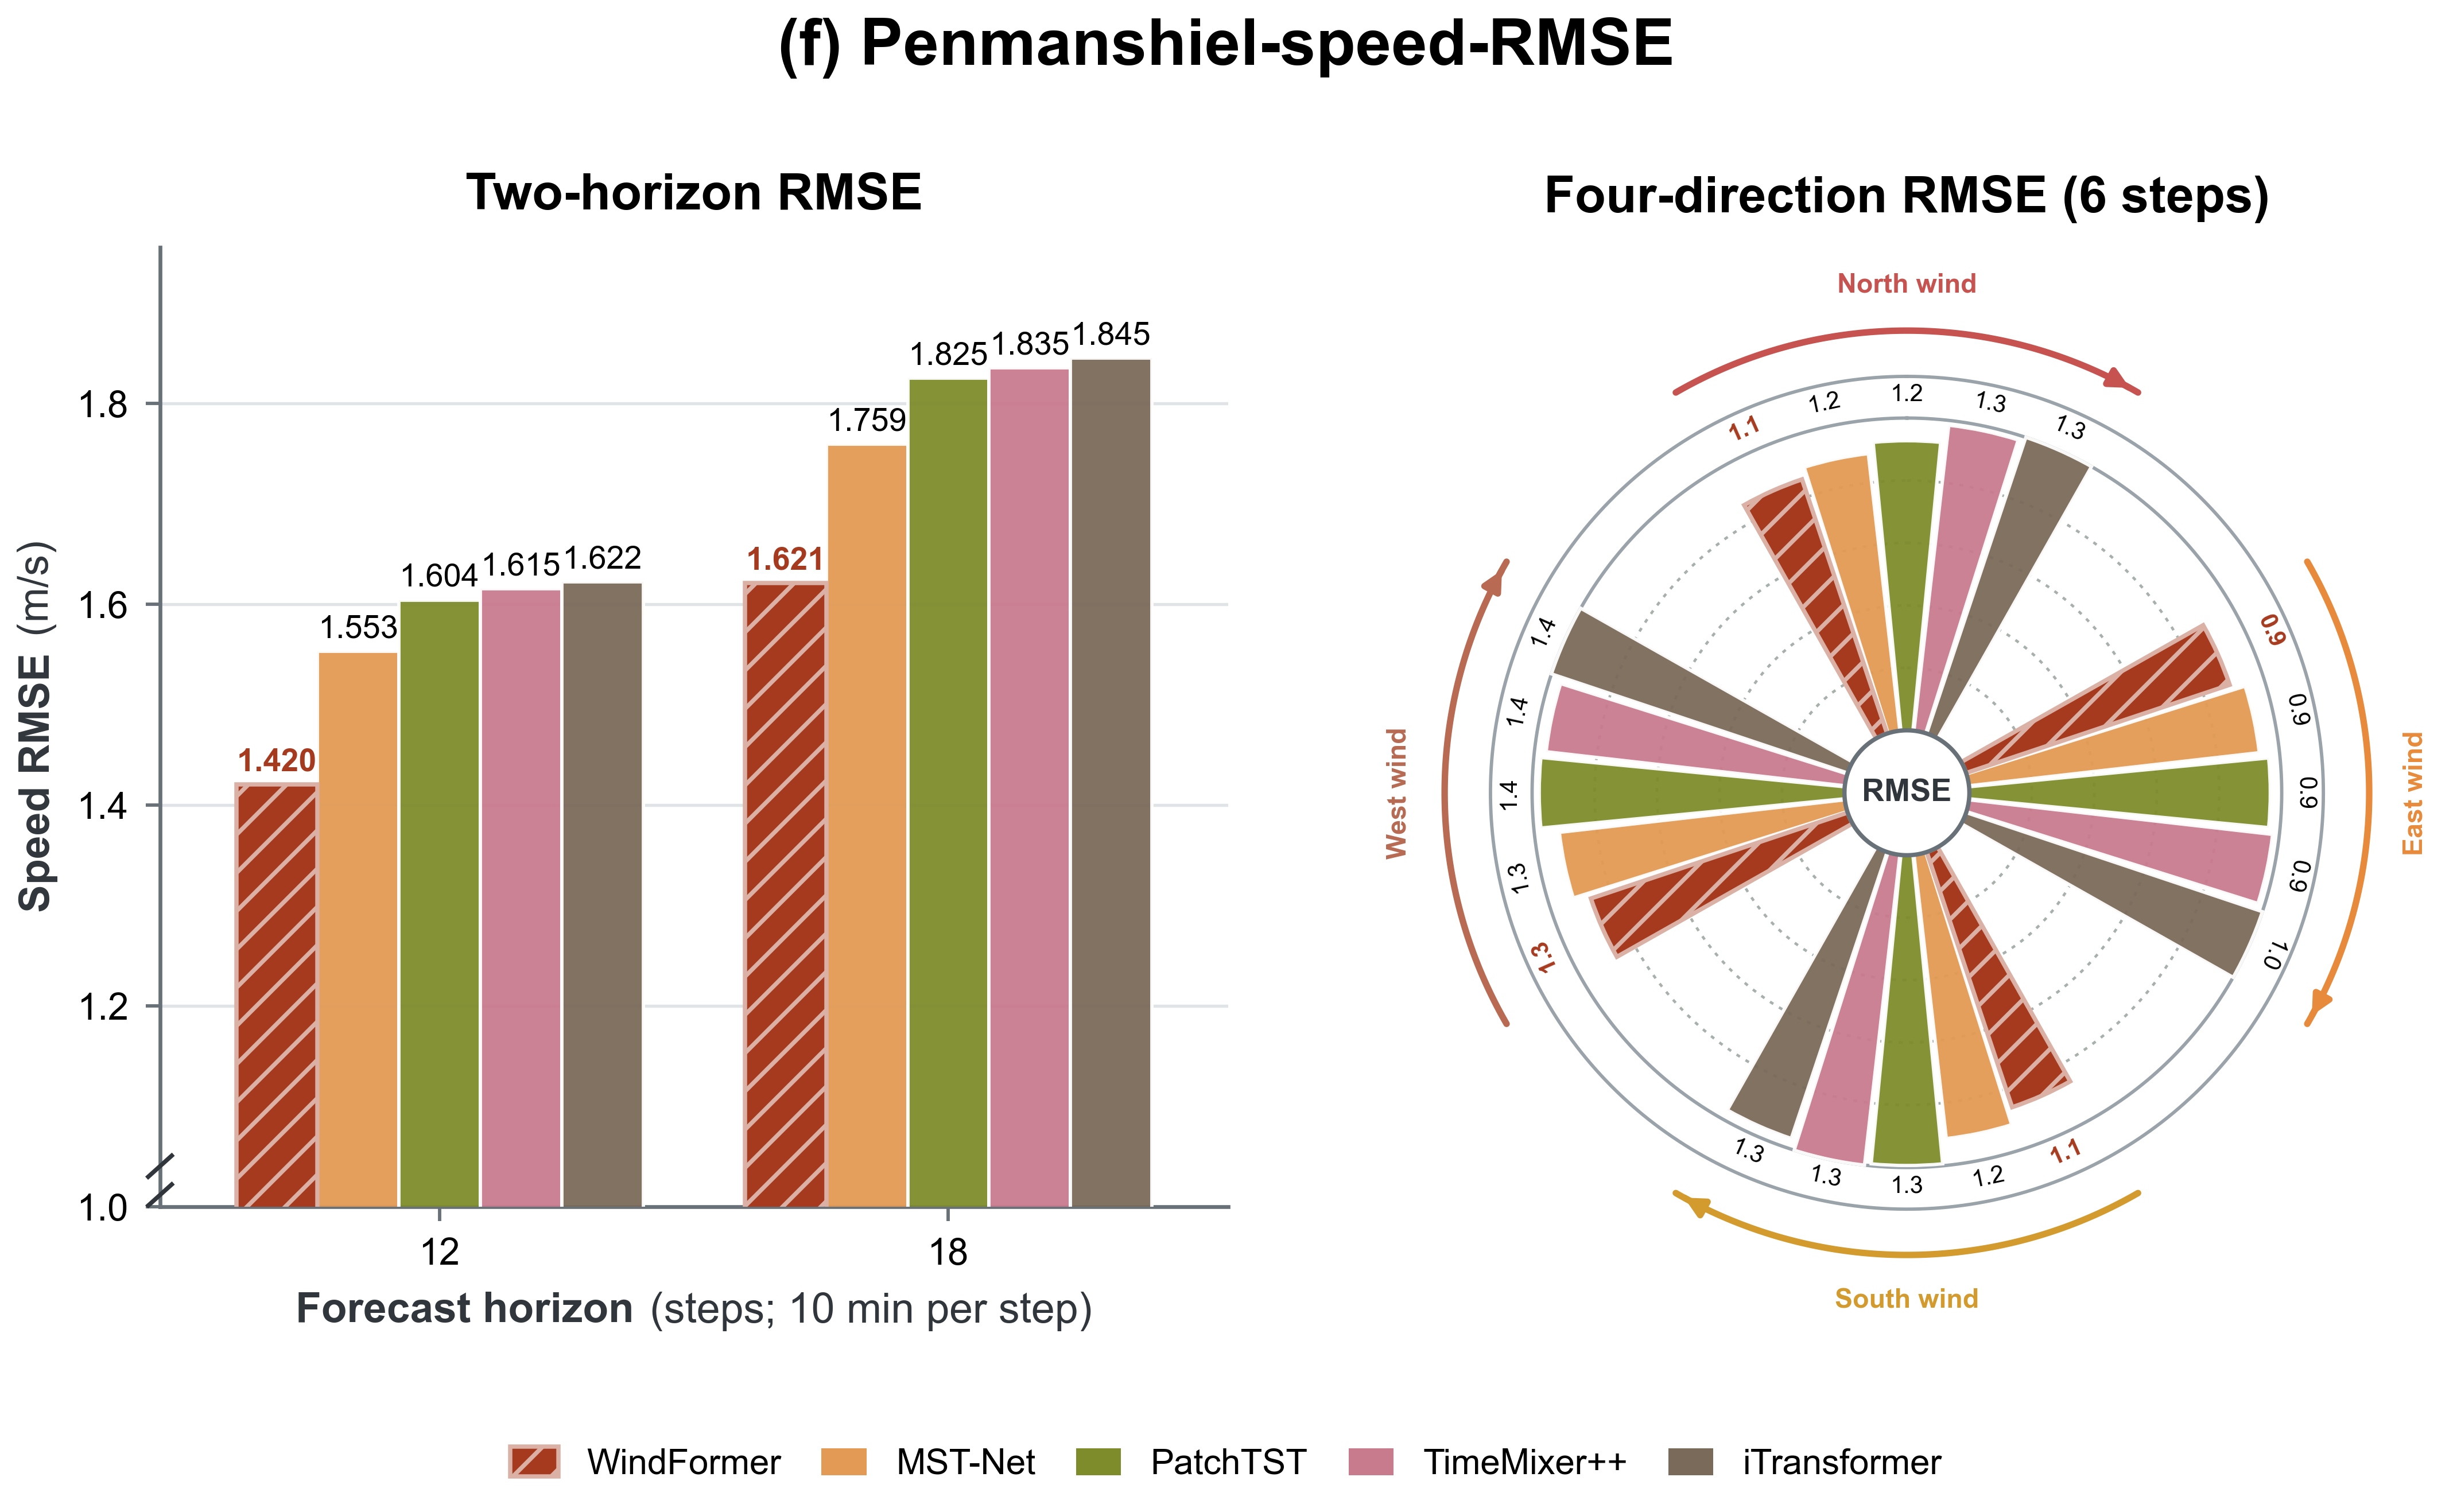
\includegraphics[width=0.49\textwidth]{figures/fig_penmanshiel_speed_rmse.png} \\[1pt]
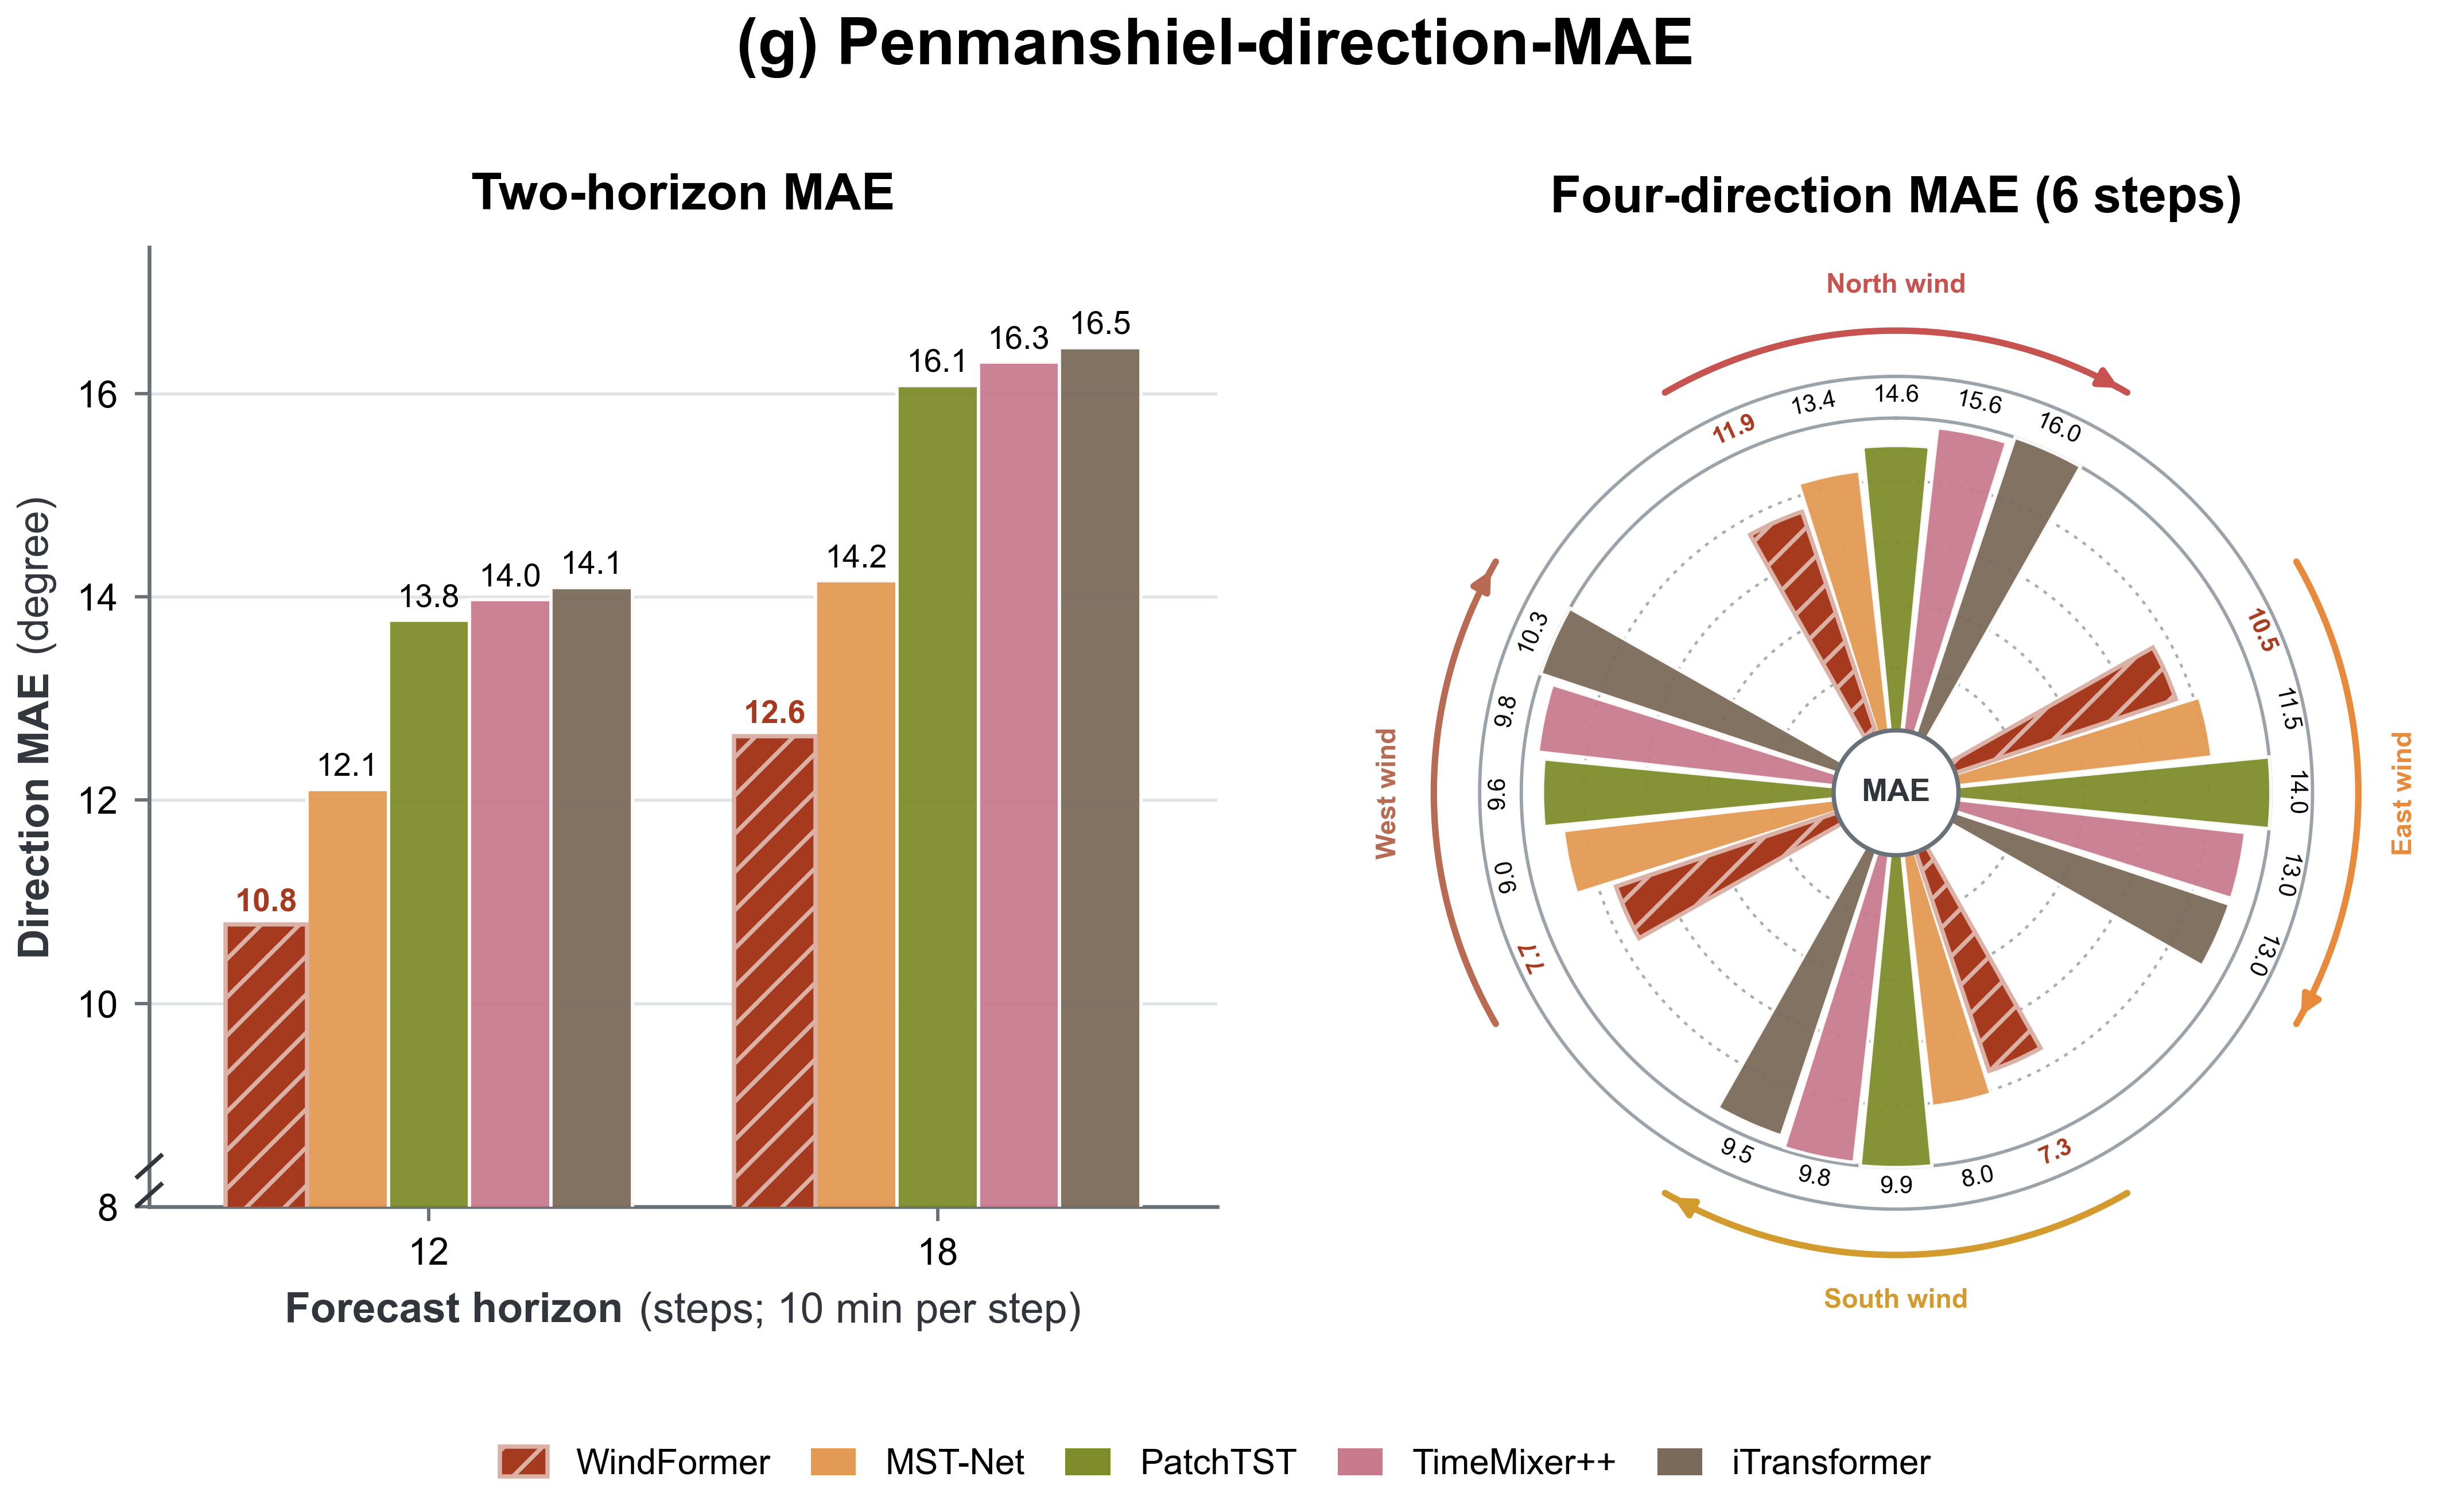
\includegraphics[width=0.49\textwidth]{figures/fig_penmanshiel_direction_mae.png} &
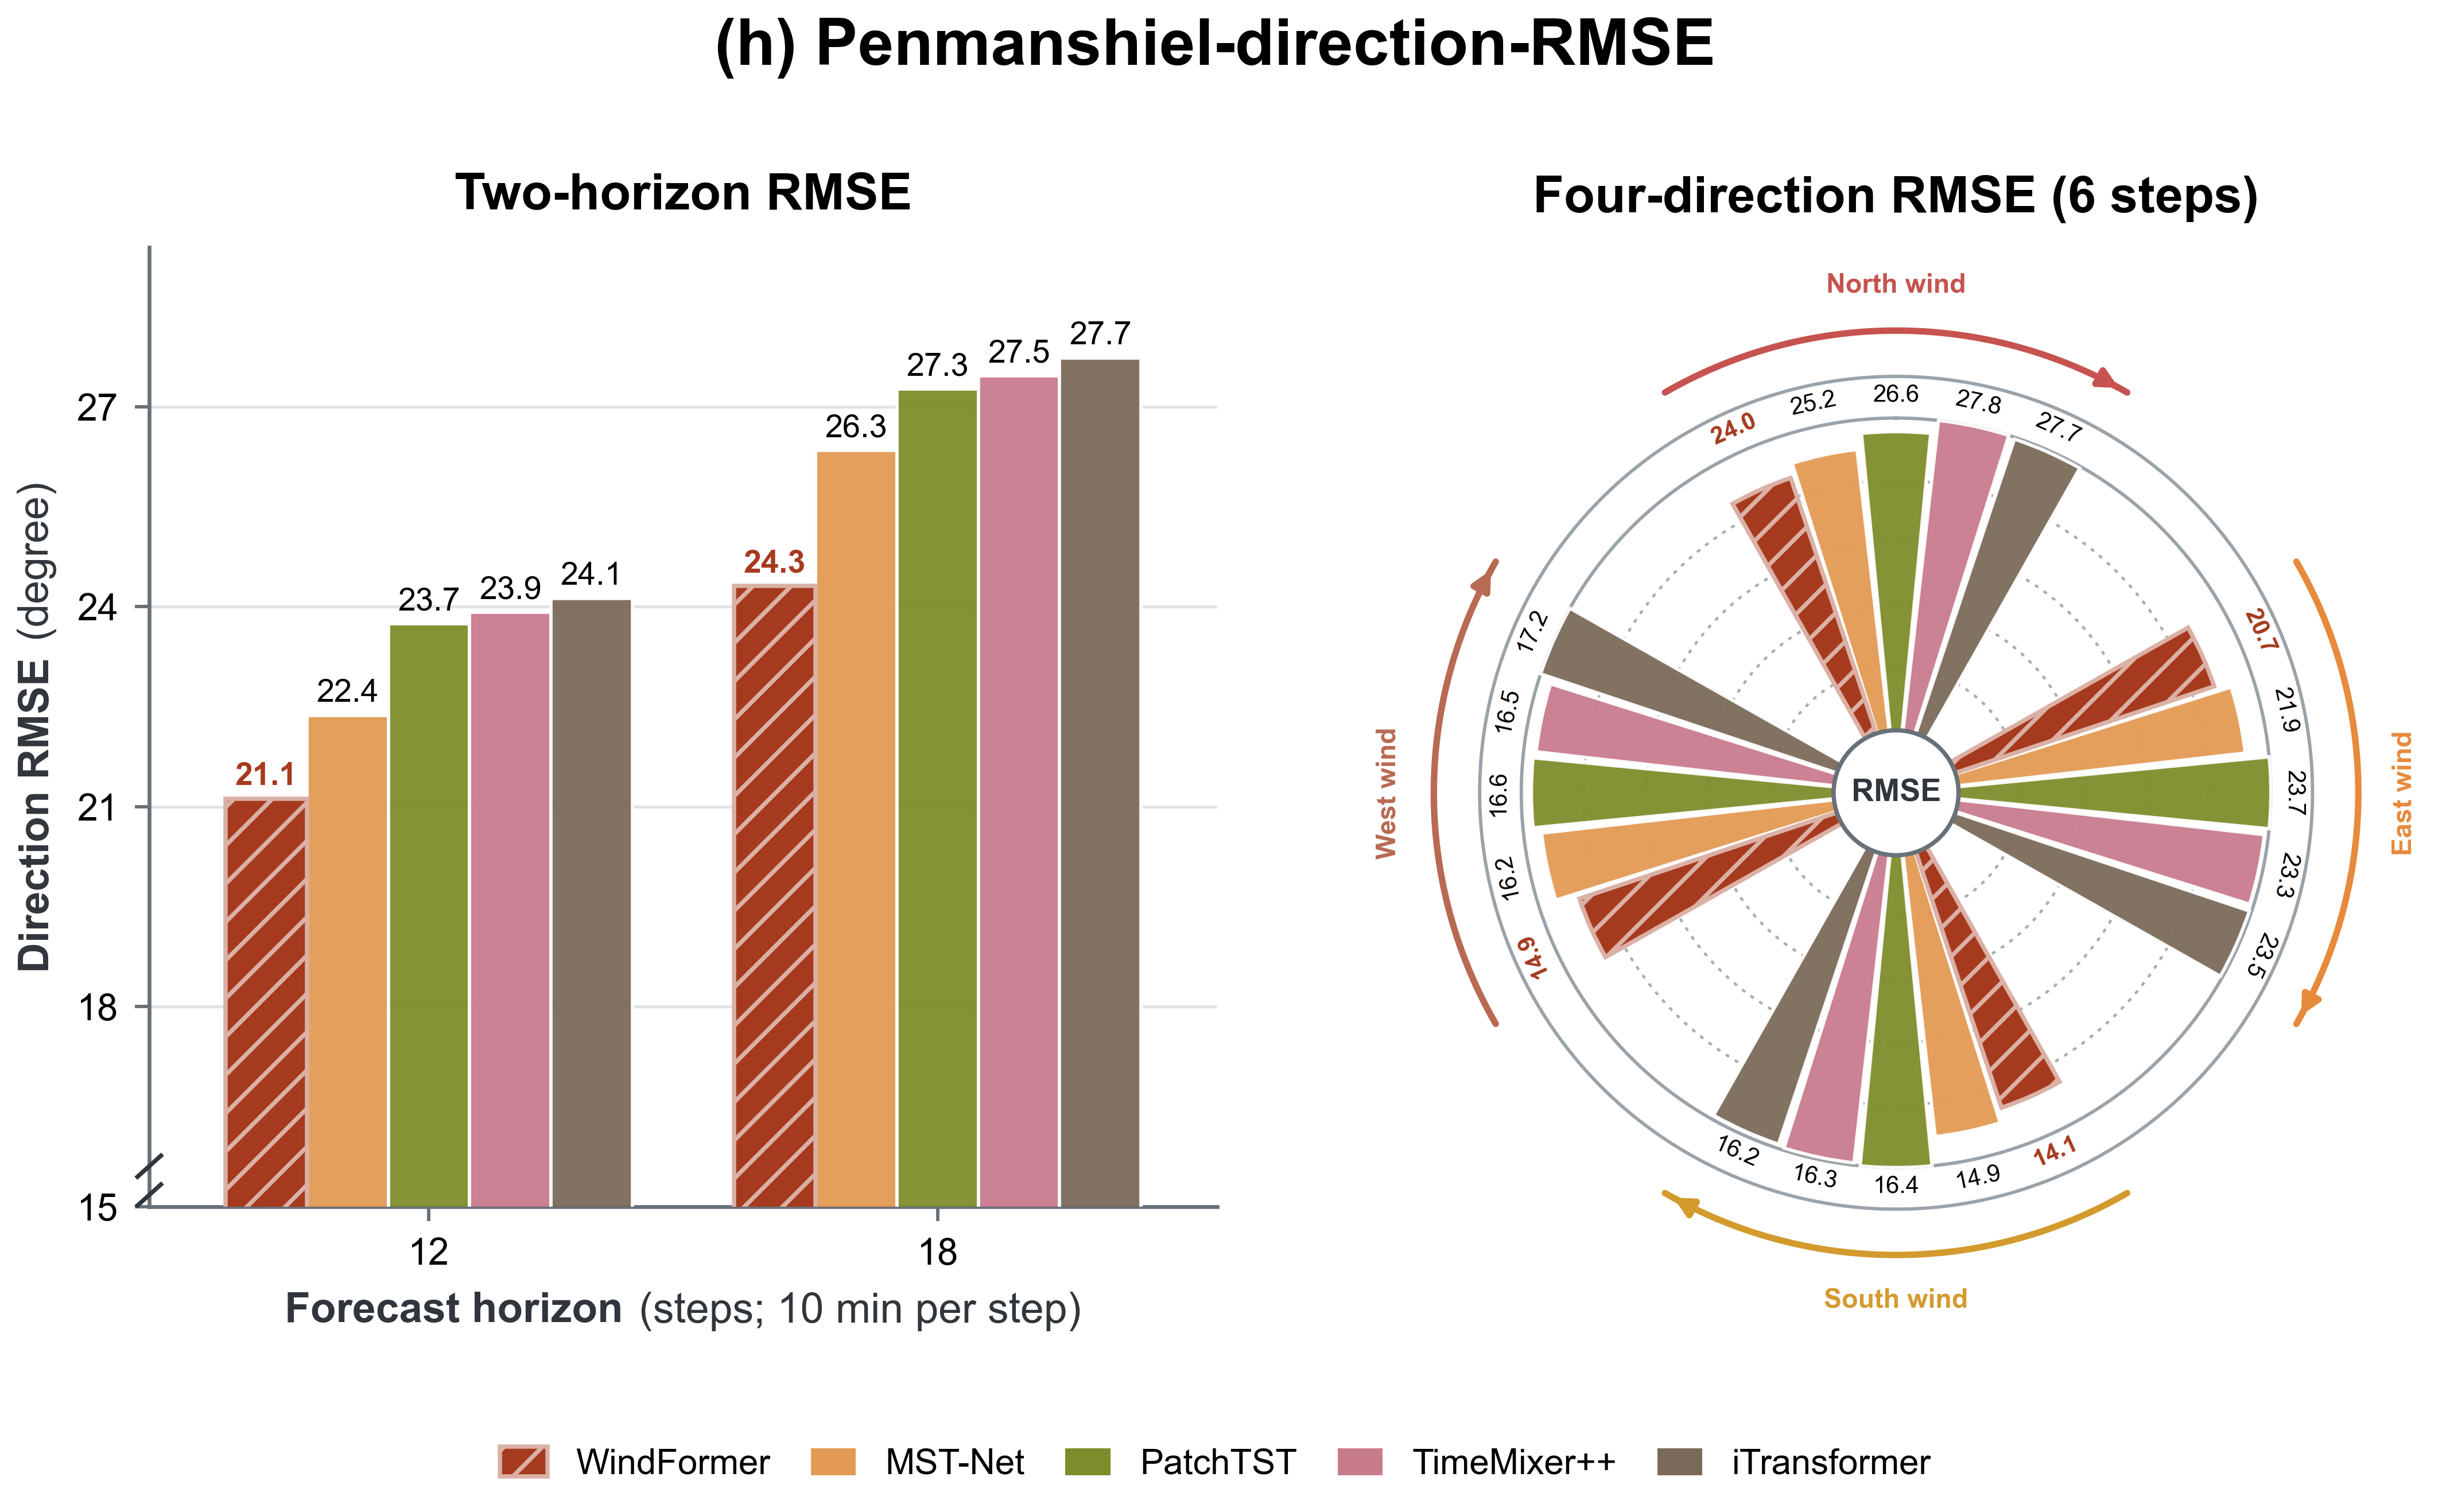
\includegraphics[width=0.49\textwidth]{figures/fig_penmanshiel_direction_rmse.png}
\end{tabular}
\vspace{-8pt}
\caption{Direction-aware forecasting results across the Shanxi and Penmanshiel wind farms. Each panel reports the two-horizon error comparison and four-direction error profile for one dataset--metric pair.}
\label{fig:formal_direction_aware_results}
\end{figure}

Figure~\ref{fig:formal_direction_aware_results} shows that the advantage is not restricted to a single aggregate score: the error profiles remain favorable across wind directions, wind variables, datasets, and reported metrics.

\begin{figure}[htbp]
\centering

\includegraphics[width=0.80\textwidth]{figures/result.png}
\caption{Representative 12-step full-sample prediction examples for wind speed and wind direction.}
\label{fig:prediction_examples}
\end{figure}

The representative forecasts in Fig.~\ref{fig:prediction_examples} further illustrate that WindFormer follows the shared trajectory while retaining turbine-level variation in the predicted signals.

\begin{table}[htbp]
\caption{Computational efficiency comparison at the 12-step forecasting horizon.}
\label{tab:efficiency}
\centering
\scriptsize
\setlength{\tabcolsep}{2.0pt}
\renewcommand{\arraystretch}{1.04}
\begin{adjustbox}{max width=\columnwidth}
\begin{tabular}{@{}lccccc@{}}
\toprule
Metric & WindFormer & MSGNet & PatchTST & iTransformer & TimeMixer++ \\
\midrule
Parameters & 36,512 & 26,680,000 & 140,492 & 124,428 & 388,332 \\
Train time (s) & 143.78 & 14356.30 & 315.32 & 57.80 & 109.55 \\
Peak GPU (MB) & 74.83 & 4532.1 & 3158.9 & 109.1 & 308.9 \\
\bottomrule
\end{tabular}
\end{adjustbox}
\end{table}

Table~\ref{tab:efficiency} shows that WindFormer combines the strongest forecasting results with a compact 36,512-parameter model and low peak GPU memory in the reported comparison.

The paired tests in Table~\ref{tab:paired-t-holm} compare WindFormer against MST-Net over five matched random seeds. All eight dataset--metric comparisons remain significant after Holm correction, supporting the consistency of the observed improvements rather than attributing them to a single seed.

\begin{table}[htbp]
\centering
\caption{Statistical significance of WindFormer improvements over MST-Net across five matched random seeds. Values are mean $\pm$ sample SD. The one-sided paired $t$-test evaluates whether WindFormer has lower error; $p_{\mathrm{raw}}$ and $p_{\mathrm{Holm}}$ are the raw and Holm-adjusted values across the eight dataset--metric comparisons.}
\label{tab:paired-t-holm}
\scriptsize
\setlength{\tabcolsep}{3.2pt}
\renewcommand{\arraystretch}{1.12}
\begin{adjustbox}{max width=\textwidth}
\begin{tabular}{clccrr}
\toprule
Dataset & Metric & WindFormer & MST-Net & $p_{\mathrm{raw}}$ & $p_{\mathrm{Holm}}$ \\
\midrule
\multirow[c]{4}{*}{Shanxi} & Speed MAE & 0.8025 $\pm$ 0.0048 & 0.8939 $\pm$ 0.0072 & $2.94\times 10^{-5}$ & $1.76\times 10^{-4}$\\
& Speed RMSE & 1.2374 $\pm$ 0.0074 & 1.3033 $\pm$ 0.0105 & $4.22\times 10^{-4}$ & $6.60\times 10^{-4}$\\
& Direction MAE & 0.3441 $\pm$ 0.0027 & 0.3806 $\pm$ 0.0038 & $3.56\times 10^{-5}$ & $1.76\times 10^{-4}$\\
& Direction RMSE & 0.6525 $\pm$ 0.0052 & 0.7041 $\pm$ 0.0070 & $3.30\times 10^{-4}$ & $6.60\times 10^{-4}$\\
\addlinespace
\multirow[c]{4}{*}{Penmanshiel} & Speed MAE & 0.8812 $\pm$ 0.0053 & 0.9879 $\pm$ 0.0078 & $3.02\times 10^{-6}$ & $2.41\times 10^{-5}$\\
& Speed RMSE & 1.4211 $\pm$ 0.0085 & 1.5538 $\pm$ 0.0124 & $1.73\times 10^{-5}$ & $1.21\times 10^{-4}$\\
& Direction MAE & 0.1881 $\pm$ 0.0015 & 0.2113 $\pm$ 0.0021 & $3.48\times 10^{-5}$ & $1.76\times 10^{-4}$\\
& Direction RMSE & 0.3686 $\pm$ 0.0030 & 0.3905 $\pm$ 0.0039 & $1.46\times 10^{-4}$ & $4.37\times 10^{-4}$\\
\bottomrule
\end{tabular}
\end{adjustbox}
\end{table}


Together, these results answer RQ1 affirmatively. WindFormer improves accuracy across both wind variables and datasets while remaining computationally compact and statistically consistent across matched seeds.

\subsection{RQ2: Which Structural Components Drive the Improvements?}
\label{subsec:ablation}

RQ2 examines whether the gains are attributable to the components introduced for the two challenges rather than to model capacity alone. The ablations therefore remove the learnable common-field weights, the circular direction representation, the wind-vector consistency loss, or the Phase-Attention temporal organization.

\begin{table}[htbp]
\caption{Ablation study results for different variants on the Shanxi and Penmanshiel datasets.}
\label{tab:ablation}
\centering
\scriptsize
\setlength{\tabcolsep}{3.2pt}
\renewcommand{\arraystretch}{1.08}
\begin{adjustbox}{max width=\textwidth}
\begin{tabular}{l|cccc|cccc|cccc|cccc}
\toprule
\multirow{3}{*}{Variant}
& \multicolumn{4}{c|}{Shanxi-6steps}
& \multicolumn{4}{c|}{Shanxi-12steps}
& \multicolumn{4}{c|}{Penmanshiel-6steps}
& \multicolumn{4}{c}{Penmanshiel-12steps} \\
\cline{2-17}
& \multicolumn{2}{c}{Speed} & \multicolumn{2}{c|}{Wdir}
& \multicolumn{2}{c}{Speed} & \multicolumn{2}{c|}{Wdir}
& \multicolumn{2}{c}{Speed} & \multicolumn{2}{c|}{Wdir}
& \multicolumn{2}{c}{Speed} & \multicolumn{2}{c}{Wdir} \\
\cline{2-17}
& MAE & RMSE & MAE & RMSE
& MAE & RMSE & MAE & RMSE
& MAE & RMSE & MAE & RMSE
& MAE & RMSE & MAE & RMSE \\
\midrule
WindFormer
& \textbf{0.6367} & \textbf{0.9884} & \textbf{0.2717} & \textbf{0.5530}
& \textbf{0.8025} & \textbf{1.2374} & \textbf{0.3441} & \textbf{0.6525}
& \textbf{0.7142} & \textbf{1.1497} & \textbf{0.1456} & \textbf{0.2914}
& \textbf{0.8812} & \textbf{1.4211} & \textbf{0.1881} & \textbf{0.3686} \\
w/o Learnable Weights
& 0.6754 & 1.0421 & 0.2765 & 0.5601
& 0.8465 & 1.3012 & 0.3495 & 0.6612
& 0.7589 & 1.2185 & 0.1502 & 0.2985
& 0.9325 & 1.5052 & 0.1935 & 0.3768 \\
w/o Direction Vector Rep.
& 0.6502 & 1.0065 & 0.6214 & 1.0851
& 0.8188 & 1.2615 & 0.7245 & 1.2562
& 0.7285 & 1.1712 & 0.4985 & 0.8124
& 0.8985 & 1.4485 & 0.5642 & 0.9351 \\
w/o Wind Vector Cons.
& 0.6612 & 1.0215 & 0.2985 & 0.5921
& 0.8315 & 1.2825 & 0.3852 & 0.7124
& 0.7412 & 1.1921 & 0.1685 & 0.3341
& 0.9125 & 1.4721 & 0.2185 & 0.4215 \\
Phase-Attn to Patch
& 0.6845 & 1.0563 & 0.2798 & 0.5644
& 0.8582 & 1.3155 & 0.3541 & 0.6658
& 0.7695 & 1.2312 & 0.1534 & 0.3018
& 0.9458 & 1.5215 & 0.1972 & 0.3812 \\
\bottomrule
\end{tabular}
\end{adjustbox}
\end{table}

Table~\ref{tab:ablation} supports the intended division of labor. Removing the direction-vector representation mainly harms direction prediction, whereas removing the learnable common-field weights or replacing Phase-Attention with ordinary patches affects wind-speed prediction more strongly. Removing the wind-vector consistency term degrades both tasks, consistent with its role as the objective-level coupling between the two branches.

\subsection{Hyperparameter Sensitivity Analysis}
\label{subsec:hyperparameter_sensitivity}

We further evaluate the sensitivity of WindFormer to four capacity and receptive-field choices: the historical input window length, the Phase Token projection dimension, the hidden dimension of the shared residual MLP, and the number of direction-branch Transformer layers. The results are summarized in Fig.~\ref{fig:hyperparameter_sensitivity}. Across all four metrics, the default configuration remains close to the best-performing setting, indicating that the structural design is not dependent on a narrow hyperparameter choice.

\begin{figure}[htbp]
\centering

\includegraphics[width=0.82\textwidth]{figures/hyperparameter_sensitivity.png}
\caption{Hyperparameter sensitivity analysis on the Shanxi dataset. The four panels vary the historical window length, Phase Token projection dimension, shared residual MLP width, and direction-branch Transformer depth.}
\label{fig:hyperparameter_sensitivity}
\end{figure}

These results answer RQ2 by linking each component to the challenge it was designed to address, while showing that the complete model does not depend on a single finely tuned capacity setting.

\subsection{RQ3: Is WindFormer Robust under Noisy and Extreme Conditions?}
\label{subsec:robustness}

RQ3 evaluates whether the structure-aware design remains useful when the inputs deviate from the clean training distribution. We consider sensor perturbations and increasing extreme-volatility severity.

For sensor perturbation, let $\theta_{i,t}$ denote the wind direction of turbine $i$ at time $t$, and let $\mathcal{W}(\cdot)$ wrap angles to the valid range. Only the wind-direction channel in the training inputs is corrupted as
\begin{equation}
\tilde{\theta}_{i,t}^{(\sigma)}=\mathcal{W}\left(\theta_{i,t}+\epsilon_{i,t}^{(\sigma)}\right),\quad
\epsilon_{i,t}^{(\sigma)}\sim\mathcal{N}(0,\sigma^2),
\label{eq:sensor_noise}
\end{equation}
where $\sigma\in\{0.1,0.2,0.3\}$ rad. Test inputs and labels remain unchanged, and all models are retrained at each noise level.

\begin{figure}[htbp]
\centering

\includegraphics[width=0.80\textwidth]{figures/supp_sensor_robustness.png}
\caption{Sensor Perturbation Robustness. The comparison covers all models, both wind speed and wind direction, and both datasets. Each subplot uses its own vertical scale to preserve dataset-specific variation.}
\label{fig:sensor_perturbation}
\end{figure}

The second experiment evaluates gust-like transient fluctuations through an EVT-inspired residual stratification scheme \cite{Pickands1975StatisticalInferenceUsingExtremeOrderStatistics,Cleveland1990STLSeasonalTrendDecomposition}. For a target series $y_t$, seasonal-trend decomposition using LOESS gives
\begin{equation}
y_t=T_t+S_t+R_t,
\end{equation}
where $T_t$, $S_t$, and $R_t$ denote the trend, seasonal, and residual terms, respectively. The extreme threshold is estimated only from the training split:
\begin{equation}
u=Q_{0.99}\left(\{|R_t|:t\in\mathcal{T}_{\mathrm{train}}\}\right),
\end{equation}
where $Q_{0.99}(\cdot)$ is the 99th percentile. A time step is identified as an extreme event when
\begin{equation}
I_t=\mathbb{I}(|R_t|>u).
\end{equation}
Given an input window of length $L=288$ ending at time $t$, the volatility severity of the corresponding forecasting sample is quantified by
\begin{equation}
N_{\mathrm{extreme}}(t)=\sum_{\tau=t-L+1}^{t}I_{\tau}.
\end{equation}
Test samples are binned by $N_{\mathrm{extreme}}(t)$ and evaluated with the trained model held fixed.

\begin{figure}[htbp]
\centering

\includegraphics[width=0.80\textwidth]{figures/supp_extreme_stress.png}
\caption{Extreme Volatility Stress Test on the Penmanshiel dataset. The figure reports wind speed and wind direction errors under increasing values of $N_{\mathrm{extreme}}$.}
\label{fig:extreme_stress}
\end{figure}

Figures~\ref{fig:sensor_perturbation} and \ref{fig:extreme_stress} show that WindFormer experiences the smallest degradation under both sensor noise and increasing extreme residual severity. This suggests that separating shared dynamics from local variation and respecting directional geometry remains beneficial when the input distribution is perturbed.

These results answer RQ3 affirmatively: WindFormer retains a more stable error profile as measurement noise and transient volatility increase.

\subsection{RQ4: Can WindFormer Generalize to Unseen Turbines?}
\label{subsec:zero_shot}

RQ4 tests whether the shared temporal parameters can transfer beyond the turbines observed during training. We conduct the \emph{Sparse Deployment Zero-Shot Evaluation} on Penmanshiel. Let $\mathcal{V}$ denote all turbines and $\mathcal{S}_k\subset\mathcal{V}$ the four turbines randomly selected in trial $k$. The remaining turbines
\begin{equation}
\mathcal{U}_k=\mathcal{V}\setminus\mathcal{S}_k
\end{equation}
are treated as unseen zero-shot targets. For a model $f_{\phi}$, $\phi$ is trained only on $\mathcal{D}_{\mathrm{train}}(\mathcal{S}_k)$ and evaluated on $\mathcal{D}_{\mathrm{test}}(\mathcal{U}_k)$. The reported error is averaged over three independent trials:
\begin{equation}
\mathrm{Err}_{\mathrm{ZS}}=\frac{1}{3}\sum_{k=1}^{3}\mathrm{Err}\left(f_{\phi_k},\mathcal{D}_{\mathrm{test}}(\mathcal{U}_k)\right).
\end{equation}
Three conditions are compared: full-sample training, zero-shot transfer, and zero-shot transfer with 0.3-rad angular noise.

\begin{figure}[htbp]
\centering

\includegraphics[width=0.80\textwidth]{figures/supp_sparse_zero_shot.png}
\caption{Sparse Deployment Zero-Shot Evaluation on Penmanshiel. The figure compares full-sample training, zero-shot transfer, and zero-shot transfer under sensor noise across multiple forecast horizons.}
\label{fig:sparse_zero_shot}
\end{figure}

Figure~\ref{fig:sparse_zero_shot} shows that WindFormer has the smallest zero-shot degradation, with a 17.72\% increase in direction MAE under the clean setting and a 15.61\% increase under 0.3-rad noise. The result indicates that shared temporal parameters and geometry-aware direction modeling can transfer to turbines that were not used as training targets.

Thus, RQ4 is answered affirmatively. WindFormer provides the strongest cross-turbine transfer among the compared models under the tested sparse-deployment conditions.
